\documentclass[12pt,a4paper,final]{report}

\usepackage{pdfpages}
\usepackage{fancyhdr}
\usepackage{amsmath}
\usepackage{graphicx}
\usepackage[hidelinks]{hyperref}
\usepackage{geometry}
\usepackage{setspace}
\usepackage{bookmark}
\usepackage{titlesec}
\usepackage{datatool}
\usepackage{tikz}
\usepackage{textcomp} % For \MakeUppercase
\usepackage[backend=bibtex, style=numeric]{biblatex}
\usepackage{glossaries} % For creating an index of abbreviations
\usepackage{longtable} % For tables that span multiple pages
\usepackage{xcolor}
\usepackage{subcaption} % for subfigures
\usepackage{pgfplots}
\usepackage{pgfplotstable}
\usepackage{multirow}

\pgfplotsset{compat=1.17}

% for creating diagrams and flowcharts
\usetikzlibrary{shapes.geometric, arrows, positioning}

% Define a custom dark green color
\definecolor{darkgreen}{rgb}{0.0, 0.5, 0.0}

\tikzstyle{startstop} = [circle, minimum width=1cm, minimum height=1cm, text centered, draw=red, fill=none, text width=1.5cm, line width=1pt, inner sep=0pt]
\tikzstyle{nodepage} = [circle, minimum width=0.25cm, minimum height=0.25cm, text centered, draw=red, fill=none, text width=0.5cm, line width=1pt, inner sep=0pt]
\tikzstyle{process} = [rectangle, minimum width=3cm, minimum height=1cm, text centered, draw=cyan, fill=none, text width=5cm]
\tikzstyle{processorange} = [rectangle, minimum width=3cm, minimum height=1cm, text centered, draw=orange, fill=none, text width=5cm, line width=1pt]
\tikzstyle{decision} = [diamond, minimum width=1cm, minimum height=1cm, text centered, draw=darkgreen, fill=none, text width=3.5cm, line width=1pt, inner sep=0pt]
\tikzstyle{coordinate} = [circle, minimum size=1pt, fill=black, inner sep=0pt]
\tikzstyle{arrow} = [thick,->,>=stealth]

% Specify line-spacing to 1.5
\onehalfspacing

% Specify margin
\geometry{top=2.5cm,bottom=2.5cm,left=3cm,right=2cm,headheight=14.5pt}

% Adjust \chapter margins
\titlespacing*{\chapter}{0pt}{0pt}{10pt} % Adjust these values as needed


% Add header and footer
\pagestyle{fancy}
\fancyhf{} % Clear all header and footer fields
% Redefine \chaptermark to remove the period after the chapter number
\renewcommand{\chaptermark}[1]{%
  \markboth{\it{\MakeUppercase{Chapter \thechapter:\ #1}}}{}}
\fancyhead[R]{\leftmark} % Left-align the chapter name
\fancyfoot[R]{Page \thepage} % Right-align page number in the footer
% Remove header line
\renewcommand{\headrulewidth}{0pt}


% Ensuring plain pages (like chapter starting pages) also use the fancy style
\fancypagestyle{plain}{
    \fancyhf{} % Clear all header and footer fields
    \fancyfoot[R]{Page \thepage} % Right-align page number in the footer
    \renewcommand{\headrulewidth}{0pt} % Remove header line on plain pages
}
\pagenumbering{Roman}

% Change Chapter formatting
\titleformat{\chapter}[hang]
    {\normalfont\huge\bfseries}
    {\thechapter}
    {1em}
    {}

% Add bibliography resources
\addbibresource{references.bib}

% Redefine \@dottedtocline to remove dots in \tableofcontents
\makeatletter
\renewcommand{\@dottedtocline}[5]{%
  \ifnum #1>\c@tocdepth \else
    \vskip \z@ \@plus.2\p@
    {\leftskip #2\relax \rightskip \@tocrmarg \parfillskip -\rightskip
     \parindent #2\relax\@afterindenttrue
     \interlinepenalty\@M
     \leavevmode
     \@tempdima #3\relax
     \advance\leftskip \@tempdima \null\nobreak\hskip -\leftskip
     {#4}\nobreak
     \leaders\hbox{} \hfill \nobreak
     \hb@xt@\@pnumwidth{\hfil\normalfont \normalcolor #5}%
     \par}%
  \fi}
\makeatother

% Get numbered subsection
\setcounter{secnumdepth}{2}

% Set the depth of the table of contents
\setcounter{tocdepth}{2}

% Start thesis
\begin{document}

% Title according to guidelines
\includepdf[pages={1,2}]{Pre-introduction/abschlussarbeit_titel-1.pdf}

\title{Robotic Workcell for Automated Bending Process}

\author{Shivam Shivam}

\date{July 2024}

%Abstract
\begin{abstract}

    This thesis demonstrates the use of a robotic workcell for
    the automation of a bending machine. The main objectives
    are to automate the bending process of a AMADA bending machine and
    enhance accuracy of bent sheets.
    The robotic workcell consists of a
    7-axis collaborative robot, two VISOR\textsuperscript{\textregistered}
    vision sensors, and a web-based UI. The robotic arm is used for the automatic
    loading and unloading of metal sheets in the bending machine.
    To achieve this, a VISOR\textsuperscript{\textregistered} camera is mounted
    on the robot for sheet detection and robotic perception. The second VISOR\textsuperscript{\textregistered}
    is used for the angle measurement of bent part and quality control.
    A web-based UI monitors the robot movement in the workcell which
    acts as a digital twin. 
    The benefits include reduction in manual labor and increased
    throughput, with improved precision and efficiency.
    This work provides valuable insights for the rapid development
    and deployment in the industry automation.
    
\vspace{1em}
\noindent \textbf{Keywords:} Robotic Workcell, Automation, 
Metal Sheet Bending, 7-axis robotic arm, VISOR\textsuperscript{\textregistered}
Computer Vision, ROS, Web UI,
Digital Twin
    
\end{abstract}



%Table of contents and other information
\tableofcontents
\listoffigures
\listoftables
% \chapter*{Symbols and Formulas}

\begin{table}[h]
\centering
\begin{tabular}{c@{\hspace{1cm}}c@{\hspace{1cm}}c@{\hspace{0.5cm}}|@{\hspace{0.5cm}}c@{\hspace{1cm}}c@{\hspace{1cm}}c@{\hspace{0.5cm}}}
Symbol & Unit & Description & Symbol & Unit & Description \\
\hline
\hline
Data 1 & Data 2 & Data 3 \\
Data 4 & Data 5 & Data 6 \\
Data 7 & Data 8 & Data 9 \\
\hline
\end{tabular}
\label{tab:symbols}
\end{table}
\chapter*{Index of Abbreviations}

% Load the acronyms
\DTLloaddb{acronym}{Pre-introduction/acronyms.csv}

% Sort the data by the first column (short)
\DTLsort{Short}{acronym}

\begin{table}[ht]
\begin{tabular}{l@{\hspace{2cm}}p{11.5cm}}
    \DTLforeach{acronym}{\short=Short, \full=Full}{%
    \vspace{5pt} % Adjust the amount of space as needed
    \textbf{\short} & \full \\
    }
\end{tabular}
\label{tab:acronyms}
\end{table}

\chapter*{Symbols and Formulas}

\begin{table}[h]
\centering
\begin{tabular}{c@{\hspace{1cm}}c@{\hspace{1cm}}c@{\hspace{0.5cm}}|@{\hspace{0.5cm}}c@{\hspace{1cm}}c@{\hspace{1cm}}c@{\hspace{0.5cm}}}
Symbol & Unit & Description & Symbol & Unit & Description \\
\hline
\hline
Data 1 & Data 2 & Data 3 \\
Data 4 & Data 5 & Data 6 \\
Data 7 & Data 8 & Data 9 \\
\hline
\end{tabular}
\label{tab:symbols}
\end{table}
% \chapter[syms]{Symbols and Formulas}
% reset page number
\newpage
\setcounter{page}{1}
\pagenumbering{arabic}

\chapter{Introduction}
\label{chap:introduction}
\chaptermark{Introduction}

\setcounter{section}{0}
\section{Background}
\label{sec:background}
The manufacturing sector is driven by the need of increased productivity. The need
for efficiency, precision, safety and cost reduction has led to significant push towards
automation. The industrial growth is currently pushed by the Industrial 4.0: a fourth wave
of technological advancements that is connecting sensors, machines, and other
\hyperref[acro:IT]{IT} systems. These connected systems, also known as cyberphysical systems, may communicate with one 
another via common Internet-based protocols and use data analysis to self-configure, anticipate 
failure, and react to changes. Industry 4.0 is making it possible to have
flexibility in production by enabling faster and efficient processes. \cite{BAI2020107776,russmann2015industry}

There are nine pillars of technological advancements, namely big data and analytics, autonomous robots, simulation,
horizontal and vertical system integration, the industrial internet of things,
cybersecurity, the cloud, additive manufacturing, augmented reality. \cite{russmann2015industry}


\begin{figure}[h]
    \centering
    \includegraphics[width=0.75\textwidth]{1. Introduction/1.1 Background/exhibit2.png}
    \caption{Industry 4.0 is changing traditional manufacturing relationships (Source: \cite{russmann2015industry})}
    \label{fig:background-exhibit-2}
\end{figure}

Metal bending processes through an \hyperref[acro:AMADA]{AMADA} bending machine, used to rely heavily upon the
manual labor traditionally. Industry 4.0 is representing a transformation
from low skill manual labor to a sophisticated system that requires \hyperref[acro:IT]{IT}-related skills
and innovation abilities in the workforce. Robotic Automation would have less variability in product
quality and will not expose operators to physical strain and repetitive motion injuries. Collaborative robots
with vision sensors \cite{8361333} allows to have flexibility in manufacturing of metal sheets.
It means robot can be programmed to perform bending of different metal sheets when required. \cite{kassowrobotsblog}


\section{Problem Statement}
\label{sec:problem}
Manual bending of metal sheets is labor-intensive and can 
lead to human errors, resulting in inconsistent quality
and inefficiency. 
The automation of this process with a collaborative robot poses
several challenges, which includes the precise detection and processing of sheet metal parts, the accurate execution of
the bend operation and the coordination of
the robotic system with other systems in the workcell.

A bending process has five stages, namely, unloading, alignment, bending, checking and loading.
Despite advancements in robotics and automation, many automated bending cells still require manual intervention or are only partially automated. Or they use seperate robotic system to operate on one of the stage of the bending process, hence requiring multiple robotic mechanisms. The challenge with this research lies in automating all the five stages of the bending process with a single handling robot. Robotic perception is required in this case for advanced error handling and collision free path planning in the workspace.
% This robotic workcell will have automatic loading and unloading
% of metal sheets in the \hyperref[acro:AMADA]{AMADA} bending machine and will use
% computer vision to detect
% and measure the bend angle of metal sheets.
% In addition, a user-friendly interface will be developed for
% monitoring the robotic workcell.

\section{Objectives}
\label{sec:objectives}
The objectives of this research are as follows:
\begin{enumerate}
    \item Developing a cost-effective solution for the automated bending process, that could replace a human operator on the bending machine while also keeping the initial costs down. The solution should be able to handle a variety of metal sheets as a human operator would be able to, allowing for flexibility in production.
    \item Production of parts should continue non-stop without any assistance from the human operator. It means the production should't stop during off hours.
    \item The solution should have a high value of accuracy in the bending process and should be able to self-adjust bending parameters to improve the bending process automatically.
    \item There should be a possibility for remote monitoring and control of the bending process, so that human operator could visualize and program the bending process of a new sheet metal part variant from outside the production space, avoiding downtime that happens during the programming of new part.
\end{enumerate}

\section{Scope}
\label{sec:scope}
The development of an automated robotic workcell for metal sheet bending holds significant implications for the manufacturing industry. By automating this process, manufacturers can achieve higher precision and consistency in product quality, reduce the reliance on manual labor, and enhance overall production efficiency. This study contributes to the broader field of industrial automation and robotics, showcasing how advanced technologies can transform traditional manufacturing processes.

This study focuses on the design, implementation, and evaluation of a robotic workcell for the bending process using a Kassow robot. The scope includes:
\begin{itemize}
    \item Integration of computer vision systems for metal sheet detection and angle measurement.
    \item Development of control software for the robotic system.
    \item Creation of a web interface for monitoring and control.
    \item Experimental evaluation of the system's performance in a simulated industrial environment.
\end{itemize}

The study does not cover other aspects of metal fabrication or the integration of additional manufacturing processes.


\section{Outline of the Thesis}
\label{sec:structure}
The thesis is organized into nine chapters. Chapter 1 introduces the background, problem statement, objectives, significance, and scope of the study. Chapter 2 reviews existing research and technologies related to robotic automation, computer vision in manufacturing, and automated bending processes. Chapter 3 describes the design of the robotic workcell, including both hardware and software components. Chapter 4 details the integration of the Kassow robot, cameras, and other hardware components. Chapter 5 discusses the development of the control software and web interface. Chapter 6 presents the integration process and testing methodology for the robotic workcell. Chapter 7 provides the results of the experimental evaluation of the system. Chapter 8 analyzes the findings, discusses implications, and addresses potential limitations. Finally, Chapter 9 summarizes the research contributions and suggests directions for future research.





\chapter{Literature Review}
\label{chap:review}

\setcounter{section}{0}
\setcounter{subsection}{0}
\section{Robotic Automation in Manufacturing}
\label{sec:automation_2}
Industrial robots were first used for repetitive tasks and material handling.
The first industrial robot, \textbf{Unimate} was deployed by General Motors in 1961. It weighed two tons and worked on assembly lines, autonomously lifting heaving objects and welding car parts. 
Since then robots have evolved to become versatile device that can perform complex tasks, learn from experience, communicate through devices, and collaborate with human workers. \cite{firstrobot}

Industrial robots are the right solution for high-volume production process for their efficiency, uptime and quality. \cite{jrautomation} As the manufacturing industry moves smaller batch production, cobots would be much more useful and flexible in a smart workcell. Cobots are vastly more advanced and affordable than industrial robots. \cite{jrautomation2}
Common use cases of robotic automation in manufacturing include material handling \cite{gambao2012new,SKIBNIEWSKI1992251}, welding \cite{tarn2011robotic}, assembly \cite{ji2021learning}, pick-and-place \cite{shah2021design}, palletizing \cite{lee2021intelligent}, and even metal sheet bending \cite{Uhrhan1995}.

Automation is particularly useful in industrial where there is a risk for human operators.
In \cite{10381692}, robotic automation has been implemented for the manufacturing of footwears which is a hazardous environment for human workers.
In it a robotic workcell consisting of three robots is controlled and coordinated through \hyperref[acro:ROS]{ROS}.

With the \hyperref[acro:CPS]{CPS}, the machines in the robotic workcell communicate and share data with each other with which production process is improved. Also, whole production process
can be monitored remotely.\cite[page 105]{li2020robotics} With the \hyperref[acro:AM]{AM} technologies, design to production time is vastly decreased. \cite[page 116]{li2020robotics}. The benefits of automation can often outweigh the initial costs. This way Industry 4.0 is transforming manufacturing sector. 

% \cite{kassowrobotsblog} Robotic automation has revolutionized the manufacturing industry by enhancing productivity, precision, and safety. Industrial robots are capable of performing a variety of tasks such as welding, assembly, material handling, and more recently, metal sheet bending. The Kassow robot, known for its high flexibility and precision, is an example of a modern industrial robot that can be effectively integrated into automated workcells.

% Recent studies have demonstrated the benefits of robotic automation in reducing cycle times, minimizing errors, and improving product quality. For instance, Kang et al. (2017) showed how integrating robots into manufacturing lines can enhance efficiency and consistency. However, the successful implementation of robotic automation requires careful consideration of factors such as system design, control algorithms, and sensor integration.


\section{Automated Bending Processes}
\label{sec:bending_2}
Sheet metal bending is a process in which bends are formed using a combination of a punch and a die. This process is used to create large number of mechanical products such as furniture panels, shelves, cabinets, housing for electromechanical devices etc. \cite{alvaautomated}
The project partner for this thesis \textit{i.e.} \textbf{mech-tron GmbH \& Co. KG} excels in the manufacturing of housing systems for electronic and embedded equipment. In this thesis, manufacturing of one of these sheet metal housing systems will be automated by means of robotic workcell.


There are various companies in the market which offers automated bending cells. They use industrial robot to feed and bend the parts in the bending machine. \cite{mekoprint, shenchong, shopmetal} or systems to assist the bending which are called \textit{bending followers} and \textit{sheet-feeder}. \cite{guimaraes2009bending} However, using a collaborative robot to perform bending tasks is challenging. A collaborative robot generally has low payload capacity and requires better robot motion planning during bending to avoid exceeding joint torques.
In \cite{liu2022metalwiremanipulationplanning}, a cobot is used to collaborate with a bending machine to perform \hyperref[acro:3D]{3D} curving of metal wire and discusses the difficulties in holding the
part in low payload robot gripper during bending and defines the generation of optimum robot motion considering the combined task and motion level constraints.

In the article \cite{cobotfabricator}, two cobots from \hyperref[acro:UR]{UR} are used for automated bending. The cobot can perform challenging bend sequences with the help of a regrip station. In similar way, unloading station is used for regrasping purposes to change the way the cobot presents the part to the bending machine.

\subsection{ASTRO bending cell}
\label{subsec:astro}

\hyperref[acro:AMADA]{AMADA} already offers an automated solution for the bending process in means of a system called ASTRO bending cell. This system consists of a handling robot which can perform production of smaller, complex workpieces and have uniformity in production. However, press brake and the know-how of handling robot come from \hyperref[acro:AMADA]{AMADA}.
The project partner has one of these systems \textit{i.e.} ASTRO-100 II NT HDS 1030 in their production floor. 

\begin{figure}[h]
    \centering
    \includegraphics[width=\textwidth]{figures/ASTRO-100.jpg}
    \caption{ASTRO-II 100NT HDS 1030 bending cell. (Source: \cite{astro100})}
    \label{fig:astro}
\end{figure}

The ASTRO-100 II NT cell is an “island solution” that is only available in the HDS-1030 press configuration, ASTRO HP-20 loading and unloading robot, ASTRO-100 II NT bending robot and the external software ASTRO CAM.
The ASTRO-100 II NT cell. \cite{astro100} The production using this system is continuous and very fast.


The main drawback of this system is the software ASTRO-CAM, which is owned by \hyperref[acro:AMADA]{AMADA}, and offers less flexibility and requires support from \hyperref[acro:AMADA]{AMADA} for programming. Without any vision sensors, the system is not smart. It can perform repetitive tasks very fast and with very little interference from operator but without any decision-making. Also, the ASTRO robot is non-collaborative and humans cannot work alongside it.
It requires a large area on the production floor which incurs more cost.

In this thesis, this system will be compared to our robotic workcell solution which has collaborative robot and is more cost-effective.


\section{Robotic System}
\label{sec:robot_2}
The real benefit of robots is taking over the three Ds, the dull, the dirty and dangerous jobs. \cite{jordan2016robots}
The functionality of a robotic system during any step of control should include three principal performance
features in the cognitive process: perception, recognition and decision making. 
It is obvious that the autonomy of the whole robotic system directly corresponds to sensory equipment, 
processing sensory information and decision algorithms. \cite{HAVLIK2011327}

Robots systems are used in industrial environments for assembling parts, painting cars or welding operations. \cite{SathishKumar2023, Wakizako}. Robots could be arranged in assembly lines to carry out a particular repetitive task. With the development in robotic perception and algorithms, robotic systems could be placed in a workcell to perform multiple tasks sequentially.
Sensory systems plays an important role to develop intelligent robotic systems. \cite{Wakizako}. Using smart sensors, a single robotic arm could perform various tasks by making decisions.

There are various  kind of robotic arms available in the market. These include industrial robots as well as cobots. Cobots are generally more sensitive and easier to program. They are also more safe to work with humans as compared to industrial robots. Industrial robots require an enclosed space for safety reasons. However, they are more durable and the speed is high. \cite{10201199}
Robotic arm also comes in different number of \hyperref[acro:DOF]{DOF}. 6-axis robotic arms are mostly common, but an additional axis from a 7-axis cobot is advantageous in our case for collision free trajectory planning in a large workspace. 

A good example of cobot is the 7-axis cobot by Kassow Robots. This sophisticated robot can mimic human movements and offers an extensive range of motion that allows it to handle intricate tasks, navigate tight spaces, and maintain consistent product quality in an industrial setting.
These cobots not only increase efficiency and productivity but also promote safety.
They can operate in industrial environments and reduces the risks associated with humans as they are collaborative. 
With the ability to work tirelessly nonstop, theese cobots ensure continuous production and uniform quality standards.
\cite{kassowrobotsblog}

\subsection{Robot Operating System}
\label{subsec:ROS}
The Robot Operating System (ROS) is a set of software libraries and tools which help to build robot applications. 
Because it is open-source, there is flexibility where and how to use ROS, as well as the freedom to customize if it requires. \cite{rosblog}
ROS is utilized to build, control or simulate various kind of robots, from mobile robots to robotic arms. \cite{koubaa2017robot}
It could also be used in partnership with a simulation environment like Gazebo. This will fasten the development process
and also make decisions before actually buying a robot. 

In \cite{takaya2016simulation}, a simulation environment is created for mobile
robots using ROS and gazebo and later tested with the real robot, showcasing the usability of the ROS for the development process.
In \cite{qian2014manipulation}, a manipulator is simulated for the pick and place operation.
There are numerous robots build using ROS and is used extensively by both hobbyists and robotic developers and is a powerful tool.

\section{Computer Vision in Industrial Automation}
\label{sec:CV_2}
% Integrating robotics, computer vision, and a user-friendly interface into a cohesive system is critical for the successful automation of the bending process. This integration ensures that the robot can accurately detect and handle metal sheets, perform precise bending operations, and provide real-time feedback to the user.

% Studies by Patel et al. (2017) and Garcia et al. (2021) have demonstrated the benefits of such integrated systems in various manufacturing applications. The integration process involves developing robust communication protocols, ensuring synchronization between components, and optimizing the system for real-time operation. The use of open-source platforms and modular design principles can facilitate this integration and enhance system flexibility.

Computer vision (CV) techniques have played an important role in promoting the information, digitization, and intelligence of industrial manufacturing systems.
CV applications include inspection, identification and process control with precision, reliability, and scalability.
In recent years, advancements in camera technology, image processing algorithms, and \hyperref[tab:acronyms]{CV} techniques have significantly increased the capabilities of vision systems in manufacturing systems.
The most common methods of \hyperref[tab:acronyms]{CV} are feature detection, recognition, segmentation, and \hyperref[tab:acronyms]{3D} modeling. \cite{9761203}


1.One of the critical aspects of implementing computer vision in industrial settings is the ability to process and analyze images in real-time, allowing for immediate feedback and adjustment in automated processes. This capability is crucial for maintaining high production speeds while ensuring precision 2.

2D Vision Systems in Industrial Applications

2D vision systems, like the Sensopart VISION camera, are widely used in industrial automation due to their ability to capture high-resolution images and detect features on flat surfaces. These systems are particularly effective in applications such as sheet detection, where they identify edges, holes, and other critical features required for further processing 3.

The Sensopart VISION camera, known for its high accuracy and robust performance, is an example of how 2D vision systems can be applied in sheet detection. This camera is capable of detecting even subtle variations in sheet features, enabling precise alignment and processing in automated bending operations. Such systems are invaluable in ensuring that the correct sheets are used in production and that they are correctly positioned, reducing errors and improving overall process efficiency 4.

Advancements in 2D Vision and Image Processing

Recent advancements in image processing algorithms have further enhanced the functionality of 2D vision systems in industrial settings. Techniques such as edge detection, pattern recognition, and feature extraction have improved the ability to identify and classify objects with high accuracy. These developments are crucial for tasks such as detecting sheet features in complex industrial environments, where lighting conditions and surface variations can pose significant challenges 5.

Moreover, the integration of machine learning with computer vision has opened new possibilities for adaptive and intelligent systems that can learn from data and improve performance over time. This approach is particularly useful in applications where variability in the manufacturing process is high, as it allows the vision system to adapt to changes and maintain high levels of accuracy 6.

Conclusion

In conclusion, computer vision, particularly 2D vision systems like the Sensopart VISION camera, plays a critical role in industrial automation. These systems enable precise detection and processing of features on sheets, contributing to the efficiency and accuracy of automated bending processes. As technology continues to advance, the integration of more sophisticated image processing and machine learning techniques will further enhance the capabilities of vision systems in industrial applications.

This review provides a concise overview of the role of computer vision in industrial automation, with a specific focus on 2D vision systems and their applications in sheet detection, such as with the Sensopart VISION camera.

\section{User Interfaces for Industrial Systems}
\label{sec:interface_2}
% An effective user interface (UI) is crucial for monitoring and controlling robotic systems. The UI should provide real-time feedback, allow for easy control of the robot, and be accessible to users with varying levels of expertise. Web-based interfaces have gained popularity due to their accessibility and ease of deployment.

% Research by Brown et al. (2019) and Nguyen et al. (2020) has emphasized the importance of intuitive UI design in enhancing user experience and system performance. Features such as real-time visualization of robotic motion, status indicators, and interactive controls are essential for effective UI. Developing a web interface for the robotic workcell can significantly enhance its usability and facilitate remote monitoring and control.

Product development process can greatly benefit from the integration of
the digital twin models. According to \cite{SEMERARO2021103469}, digital twin (DT) embeds a "virtual" image of the reality
constantly synchronized with the real operating scenario to provide sound information (knowledge model) to reality interpretation model to draw sound decisions.

In manufacturing a digital twin can replicate an individual machine, a cell, a complete line. Digital twin and virtual commissioning are two terms that often come when
talking about Industry 4.0. Both use virtual representations of physical systems to save time, enable better training, and identify improvement opportunities, among other benefits. However, the digital twin requires a physical equivalent with \hyperref[tab:acronyms]{IoT} technology for data transfer. Virtual commissioning requires simulation of all the signals with their timings and sensors and actuator responses.
It can exist without a physical system. \cite{digitaltwinblog}

Digital twin enables the creation of high-performance products and optimize production systems by allowing early estimations and later reconfigurations. The connectivity of Industry 4.0 technologies is highlighted as a key strategy for achieving the most efficient product specifications in technical and economic terms for the manufacturer. 
Simulations with a digital production twin open up new possibilities in production integration.
\cite{WAGNER201988}


In this thesis, virtual commissioning is first accomplished in order to speed up the development process. Next step is to get the data from the real robotic system and use it to test and verify the virtual model.
This will be the digital twin model which will help in:
\begin{enumerate}
    \item Identify collision points in the real world and use it to plan trajectory.
    \item Monitor and optimize the loading and unloading process.
    \item Offer testing opportunities for a new product model.
\end{enumerate}

 Similarly, Md. Touhidul Islam et al. (2023) showcased a web-based Human-Machine Interface (HMI) for a ROS-based autonomous wheelchair, highlighting the potential of web interfaces in enhancing the usability of assistive robotics.
Versatile and accessible UI could be created using web technologies and ROS for robot control.
In this paper \cite{Xiao_2019}, a web-based interface that utilizes ROS alongside HTML5, Javascript and C++, allows for remote control, real-time monitoring, and 3D visualization of robots.


In the realm of Human-Robot Interaction (HRI), Christos Papadopoulos et al. (2018) created a web interface that enables non-experts to teach robots new assembly tasks, emphasizing the significance of user-friendly design in collaborative robotics. W. A. M. Fernando et al. (2022) developed a web-based learning environment for ROS applications that integrates with the Gazebo simulator, offering a valuable tool for both education and practical development. These studies illustrate how web-based interfaces are transforming robotic systems by making them more intuitive, accessible, and applicable across various domains.

\chapter{System Design}

\setcounter{section}{0}
\setcounter{subsection}{0}

\section{Overview of the Robotic Workcell}

\section{Hardware Selection}

\section{Software Architecture}



\chapter{Hardware Integration}
\label{chap:integration}

\setcounter{section}{0}
\setcounter{subsection}{0}

\section{Installation and Configuration}

\subsection{Robot Unit}

The robot unit consists of three assemblies: a base, a robot and a gripper (Figure \ref{fig:kr1410}).

\begin{figure}[h]
    \centering
    \includegraphics[width=\textwidth]{3. System Design/3.2 Hardware Selection/kr1410.png}
    \caption{Components of the robot unit: 1) robot base; 2) robot from kassow robots; 3) manual quick-change system; 4) pneumatic parellel gripper; 5) camera system}
    \label{fig:kr1410}
\end{figure}

The base is a simple welded construction made of steel. The choice of steel material ensures that the base has
sufficient dead weight so that it can be transported together with the robot and gripper using a pallet
truck without the risk of tipping over. During operation, the robot unit is fixed to the floor with four M12
screws. The robot used is a 7-axis robot from Kassow Robots. This fulfills the requirements defined in
the first work packages. The gripper is a pneumatic parallel gripper with a manual quick-change
system. The gripper was selected according to payload, gripping force and opening width. The
opening width is the dominant selection criterion here, as the gripper must be able to grip both the thin
sheets with thicknesses of around 1 to 3 mm and the handle on the drawers with a width of 15 mm. An
electric gripper was also considered, as the power supply could have been provided via the cable
already integrated in the robot. Due to the higher costs, the double height and the weight, a pneumatic
gripper was chosen.



The manual quick-change system makes it possible to exchange different gripper
designs in a short time and without increased effort if required for a sheet metal part type. Sheet metal
part is folded into something like a box. For this, it is technically sensible or necessary to use a
vacuum gripper.
This means that collision-free gripping is not possible with a parallel gripper after the last bend. The
quick-change system also has an electric and pneumatic power feed-through, which ensures simple,
user-friendly changeover.



Furthermore, a camera system is installed on the robot itself. This is used to determine the relative
position between the robot unit and the sheet pickup station, bending machine and storage shelf using the markers
and between the robot unit and the sheet metal part (when it is first made available at the
sheet pickup station or is gripped) using features on the sheet metal part.

\section{System Networking}
(such as TCP/IP, UDP or Modbus TCP)

\begin{figure}
    \centering
    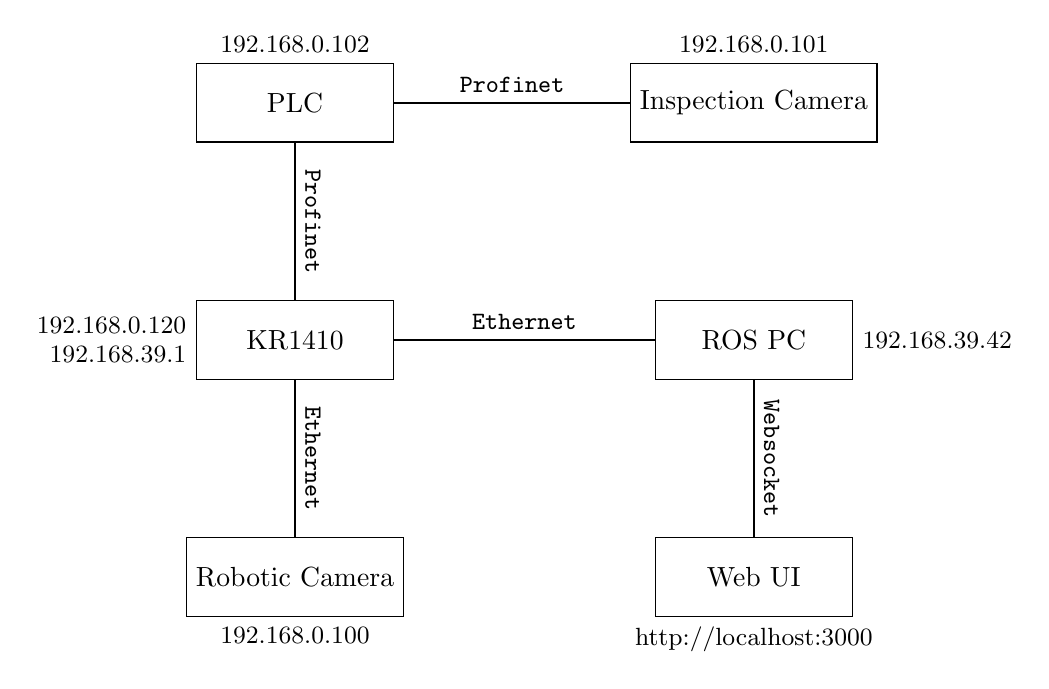
\begin{tikzpicture}[
        device/.style={draw, rectangle, minimum width=2.5cm, minimum height=1cm, align=center},
        connection/.style={thick}, % bidirectional arrows
        protocol/.style={above, sloped, font=\small\ttfamily},
        ip/.style={font=\small} % IP address style
      ]
      
      % Devices without IP inside node
      \node[device] (PLC) {PLC};
      \node[device, below=2cm of PLC] (KR1410) {KR1410};
      \node[device, right=3cm of PLC] (InspectionCamera) {Inspection Camera};
      \node[device, below=2cm of KR1410] (RoboticCamera) {Robotic Camera};
      \node[device, below=2cm of InspectionCamera] (PC) {ROS PC};
      
      % Web UI node
      \node[device, below=2cm of PC] (WebUI) {Web UI};
      
      % IP addresses outside nodes
      \node[ip, above=0.0cm of PLC] {192.168.0.102};
      \node[ip, above left=-0.55cm and 0cm of KR1410] {192.168.0.120};
      \node[ip, below left=-0.55cm and 0.0cm of KR1410] {192.168.39.1};
      \node[ip, above=0.0cm of InspectionCamera] {192.168.0.101};
      \node[ip, below=0.0cm of RoboticCamera] {192.168.0.100};
      \node[ip, right=0.0cm of PC] {192.168.39.42};
      \node[ip, below=0.0cm of WebUI] {http://localhost:3000};

      % Connections
      \draw[connection] (PLC) -- (KR1410) node[protocol, midway] {Profinet};
      \draw[connection] (KR1410) -- (RoboticCamera) node[protocol, midway] {Ethernet};
      \draw[connection] (KR1410) -- (PC) node[protocol, midway] {Ethernet};
      \draw[connection] (PLC) -- (InspectionCamera) node[protocol, midway] {Profinet};
      \draw[connection] (PC) -- (WebUI) node[protocol, midway] {Websocket};
      
      \end{tikzpicture}
    \caption{System Networking and IP Addressing}
    \label{fig:communication-protocols}
\end{figure}



\section{Safety Considerations}
Even though the robot chosen is a collaborative robot, the payload is a metal sheet which poses a safety concern for the human operator.
To avoid such scenarios a safety fence is installed at the boundary of robotic workcell as mentioned in section \ref{sub:safety-fence}.
Still several considerations are required for the safe operation of robot in the workcell like the speed at which the robot should operate. These factors depends on the payload attached to the robot and the distance between payload and the joint axis 1 or joint axis 2.
Following subsections explains the reasoning behind safety parameters that were considered for the safe operation of KR1410.

\subsection{Payload}
\label{subsec:payload}
The pneumatic parellel gripper, manual quick-change system and robotic camera constitutes a weight of 2.0 \textit{kg}.
This is the fixed load on the tool flange center (\hyperref[acro:TFC]{TFC}). The sheet metal parts counts as the payload.
It is a variable load of only 0.1 \textit{kg} and is thus ignored for the calculations in \ref{subsec:stoppage-distance}.


\begin{figure}[h]
    \centering
    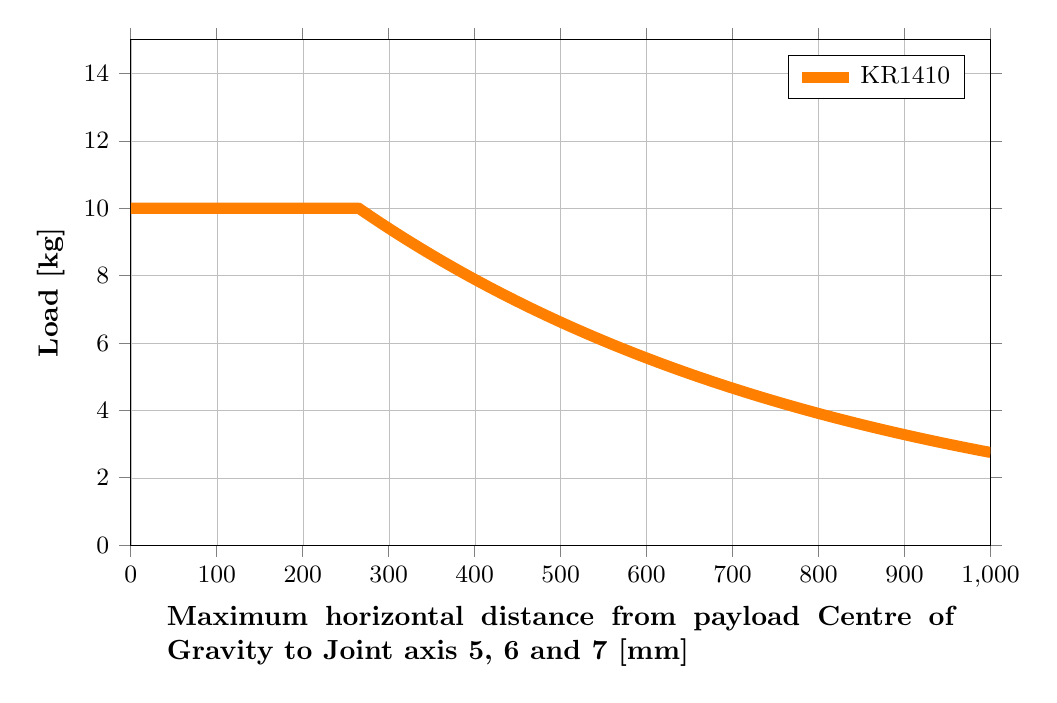
\begin{tikzpicture}
        \begin{axis}[
            width=12.5cm,
            height=8cm,
            grid=both,
            grid style={line width=.1pt, draw=gray!30},
            major grid style={line width=.1pt,draw=gray!50},
            xlabel={\parbox{10cm}{Maximum horizontal distance from payload Centre of Gravity to Joint axis 5, 6 and 7 [mm]}},
            ylabel={\textbf{Load [kg]}},
            xmin=0, xmax=1000,
            ymin=0, ymax=15,
            legend pos=north east,
            legend style={font=\small},
            ylabel near ticks,
            xlabel near ticks,
            tick align=outside,
            tick label style={font=\small},
            label style={font=\bfseries},
        ]
    
        % KR1410 (orange)
        \addplot [
            color=orange,
            line width=4pt,
            % ultra thick,
            domain=0:1000,
            samples=1000,
        ]
        {x <= 265 ? 10 : 10*exp(-0.001756*(x-265))};
        \addlegendentry{KR1410}
        \end{axis}
    \end{tikzpicture}
    
    \caption{Payload diagram for KR1410 manipulator}
    \label{fig:kr1410-payload-diagram}
\end{figure}


The permissible payload is constrained due to the static torque limit of the wrist joints. The payload is
reduced according to the proximity of the payload's centre of gravity in relation to joint axis 5, 6 and 7. \cite[page 35]{kassow-manual}
Only about 1100 \textit{mm} out of 1400 \textit{mm} of workspace is utilized by the KR in the workcell. 
Figure \ref{fig:kr1410-payload-diagram}
illustrates the allowable payload as a function of distance. It's evident from this it is safe to operate with a load a 2.0 \textit{kg}.

\subsection{Stopping Distance}
\label{subsec:stoppage-distance}
The stopping time \hyperref[sym:t-brake]{$t_{\text{brake}}$} and distance \hyperref[sym:s-brake]{$s_{\text{brake}}$} should be kept as low as possible. \hyperref[sym:s-brake]{$s_{\text{brake}}$} is set at 60 \textit{mm} and \hyperref[sym:t-brake]{$t_{\text{brake}}$} at 0.2 \textit{s} for safety reason.
According to \cite[page 35]{kassow-manual}, the time and distance it takes to stop the robot, for instance with an emergency stop or protective stop, depends on the load, speed
and configuration of the robot. Conservative estimations of \hyperref[sym:t-brake]{$t_{\text{brake}}$} and \hyperref[sym:s-brake]{$s_{\text{brake}}$} are made by firstly identifying how fast the
slowest joints can decelerate. This depends on the payload, the direction in which the payload is heading
relative to gravity, and the distance between the load or \hyperref[acro:TFC]{TFC} and joint axis 1 or 2, depending on whatever
distance is the longest.
The values can be seen in the Table \ref{tab:braking_accelerations}.


    \begin{table}[h]
        \centering
        \renewcommand{\arraystretch}{1.2} % Adjusts row height
        \small
        \setlength{\tabcolsep}{4.5pt} % Adjusts column spacing
        \begin{tabular}{cc|*{7}{c}}
            \hline
            \textbf{Load} & \textbf{Direction} & 
            \multicolumn{7}{c}{\textbf{Distance from Joint axis 1 or 2 to Load center}} \\
            \textbf{[kg]} & \textbf{[deg]} & 
            \multicolumn{7}{c}{\textbf{of gravity or TFC, whichever is larger}} \\
            \cline{3-9}
            & & 800-950 & 700-800 & 600-700 & 500-600 & 400-500 & 300-400 & 0-300 \\
            \hline
            \multirow{4}{*}{0-4}  & 0-40  & 895  & 1026 & 1304 & 1663 & 2131 & 2724 & 3437 \\
                                & 40-80 & 1433 & 1578 & 1745 & 2132 & 2522 & 3131 & 3724 \\
                                & 80-120 & 1378 & 1549 & 1720 & 2115 & 2643 & 3165 & 4045 \\
                                & 120-160 & 1861 & 2040 & 2371 & 2773 & 3259 & 3824 & 4342 \\
            \hline
        \end{tabular}
        \caption{Braking accelerations \hyperref[sym:a-brake]{$a_{\text{brake}}$} \textit{$[\text{deg/s}^2]$} for KR1410}
        \label{tab:braking_accelerations}
    \end{table}

    The stopping time \hyperref[sym:t-brake]{$t_{\text{brake}}$} and stopping distance \hyperref[sym:s-brake]{$s_{\text{brake}}$} can now be conservatively estimated based on the knowledge of the set speed
    in the robot program and equations \ref{eq:t-brake} and \ref{eq:s-brake}. Joint speed \hyperref[sym:omega]{$\omega$} is used for \hyperref[acro:Move J]{Move J} and linear speed \hyperref[sym:v-max]{$v_{\text{max}}$} for \hyperref[acro:Move L]{Move L} and \hyperref[acro:Move S]{Move S} commands.
    By default in normal run mode of program, Move J command runs a maximum joint speed of 90 \textit{deg/s} and
    Move L command runs a maximum linear speed of 1000 \textit{mm/s}. This linear speed can be converted to joint speed
    using the equation \ref{eq:omega}.

    \begin{equation}
        \omega = \frac{180 \, v_{\text{max}}}{r\pi} \quad [\text{deg} \, s^{-1}]
        \label{eq:omega}
    \end{equation}
                
    \begin{equation}
        t_{\text{brake}} = \frac{\omega}{a_{\text{brake}}} + 0.020 \quad [\text{s}]
        \label{eq:t-brake}
    \end{equation}
        
    \begin{equation}
        s_{\text{brake}} = \left(\frac{t_{\text{brake}} + 0.02}{360}\right) \pi r w \quad [\text{mm}]
        \label{eq:s-brake}
    \end{equation}

    From these equations, it is evident that \hyperref[sym:t-brake]{$t_{\text{brake}}$} and \hyperref[sym:s-brake]{$s_{\text{brake}}$} are directly proportional to \hyperref[sym:omega]{$\omega$}.
    To avoid triggering joint torque value exceeded error and for safe operation of robot, the joint speed \hyperref[sym:omega]{$\omega$} is reduced for specifically difficult trajectory execution or when the distance
    between joint axis 1 or joint axis 2 and \hyperref[acro:TFC]{TFC} is large. For example, to keep the same \hyperref[sym:t-brake]{$t_{\text{brake}}$} for a distance of 900 \textit{mm} between Joint axis 1 and payload
    but two robot configuration of 0-40 \textit{deg} and 120-160 \textit{deg}, joint speed \hyperref[sym:omega]{$\omega$} must be halved
    for 0-40 \textit{deg} robot configuration.

\subsection{Safety zones}
\label{subsec:safety-zones}

Safety Zones represent virtual boundaries in the robot workspace. The robot will reduce its speed or stop
completely if any part of the robot enters the safety zone. This can be used for protection of sensitive
equipment or areas with human presence. \cite[page 96]{kassow-software-manual}


\begin{figure}[h]
    \centering
    \includegraphics[width=0.7\textwidth]{figures/safety-zones.png}
    \caption{Addition of safety zones to the robotic workcell}
    \label{fig:safety-zones}
\end{figure}

A safety zone for unloading station, storage station, bending machine and terminal operating
robot is created. Since the
robot can actually touch the floor, an additional safety zone is added for the floor. 
The robot will stop immediately if it ever exceeds the safety zone boundary. It it exceeds, 
then the operator
has to manually move the robotic arm back inside the safety zone. 

\subsection{Safety functions}
\label{subsec:safety-functions}
Safety functions evaluate external and internal signals of the whole system which can act immediately to
halt the robot or cut him loose from power if necessary. 
The safety function of KR complies with EN ISO 13849-1:2015. \cite{ISO13849}
\cite[page 13]{kassow-software-manual}

\begin{figure}[h]
    \centering
    \includegraphics[width=0.7\textwidth]{figures/safety-buttons.png}
    \caption{Safety buttons. 1) Emergency STOP 2) Protective STOP 3) Robot State 4) Reset PLC fault}
    \label{fig:safety-buttons}
\end{figure}

In the main program of teach pendant, there are two sequences programmed to run in parallel to halt or stop the program if a signal is detected
from the PLC. The former sequence pauses the robot motion and waits for a new signal from PLC to continue the robot motion from the same configuration while the latter sequence triggers the E-Stop on the robot and stops the robot immediately. 



\subsubsection{Protective STOP}
The Protective STOP can be used interactively by the operator to pause and continue the running program.
After the protective STOP is released, the program can continue running its normal operation.

\subsubsection{Emergency STOP}
The emergency STOP buttons of robot are present at both teach pendant and robot controller. These buttons are used to engage inbuilt safety measures and halt the robot in order to
prevent a potentially hazardous situation
The emergency STOP always provoke immediate halt of the robot, followed by the power cut to all
executive parts of the robot.

Besides these E-stop buttons, there are three more E-Stop in the workcell. Two are placed on the bending machine and one on the front panel of unloading station as shown in figure \ref{fig:safety-buttons}. The emergency stop buttons not only stops the robot but also the bending machine and unloading station mechatronic system.


\vspace{1\baselineskip}



\chapter{Software Development}
\label{chap:development}

\setcounter{section}{0}
\setcounter{subsection}{0}

\section{Control Software}
By analyzing the current manual process on the bending machine, a flowchart for the mobile robot unit
is developed for the automated bending process. This
diagram, which is still partly abstract, enables the individual activities of the unit to be identified and
their interactions to be described right at the start of the research project. The requirements for the
overall system are also defined, which are explained in more detail
in subchapter \ref{sub:overview}. The description of the process and the definition of the overall requirements
represent an interacting process that inevitably had to be iterated through. This means that the results
of both work packages were revised several times. The final result of these iterations regarding the
activities to be performed by the mobile robot unit can be seen in Figure 1 and Figure 2. Five essential
components of the unit emerge from the process. These are as follows: Feeding, alignment, bending,
checking and depositing.

In the first step, the feed, the sheet metal is to be separated from a stack of sheets. The advantage of
arranging the raw sheets in stacks is that as many parts as possible can be stored in as little space as
possible. Conversely, this means that more space is available for the bent sheet metal parts, which is
of great importance due to the limited space available on site at the company. The sheet thickness is
also checked in advance during feeding and parts outside the tolerance are sorted out. Furthermore,
this information should be taken into account in the further course of the process when adjusting the
parameters of the bending machine.

For space reasons, a device should be integrated into the feeder that allows the robot to grip the sheet
metal at a new position if necessary, as otherwise collisions between the robot and the bending
machine may occur during the subsequent bending process if the robot is not realigned.
During the bending process, there should be two different design variants depending on the sheet
variant. With small sheets, the robot lets go of the sheet, which has an advantageous effect on the
robot programming. In order to prevent twisting in the case of larger parts, it is essential to hold them
throughout the entire bending process. The challenge here lies in programming a robot movement
whose path and path speed matches the movement of the sheet metal, which in turn depends on the
lowering speed of the bending punch.

A camera system is used to record both the angle and length of the sheet metal after each individual
bending process. The angle is used to readjust the bending machines. The length measurements
serve as a further instrument for monitoring the process. If a large number of rejects occur in a very
short time, the entire process is to be stopped.
The fully bent sheet metal parts are to be placed in storage boxes that are already in use in the
company but still need to be adapted.


\begin{longtable}{c}
    \small
    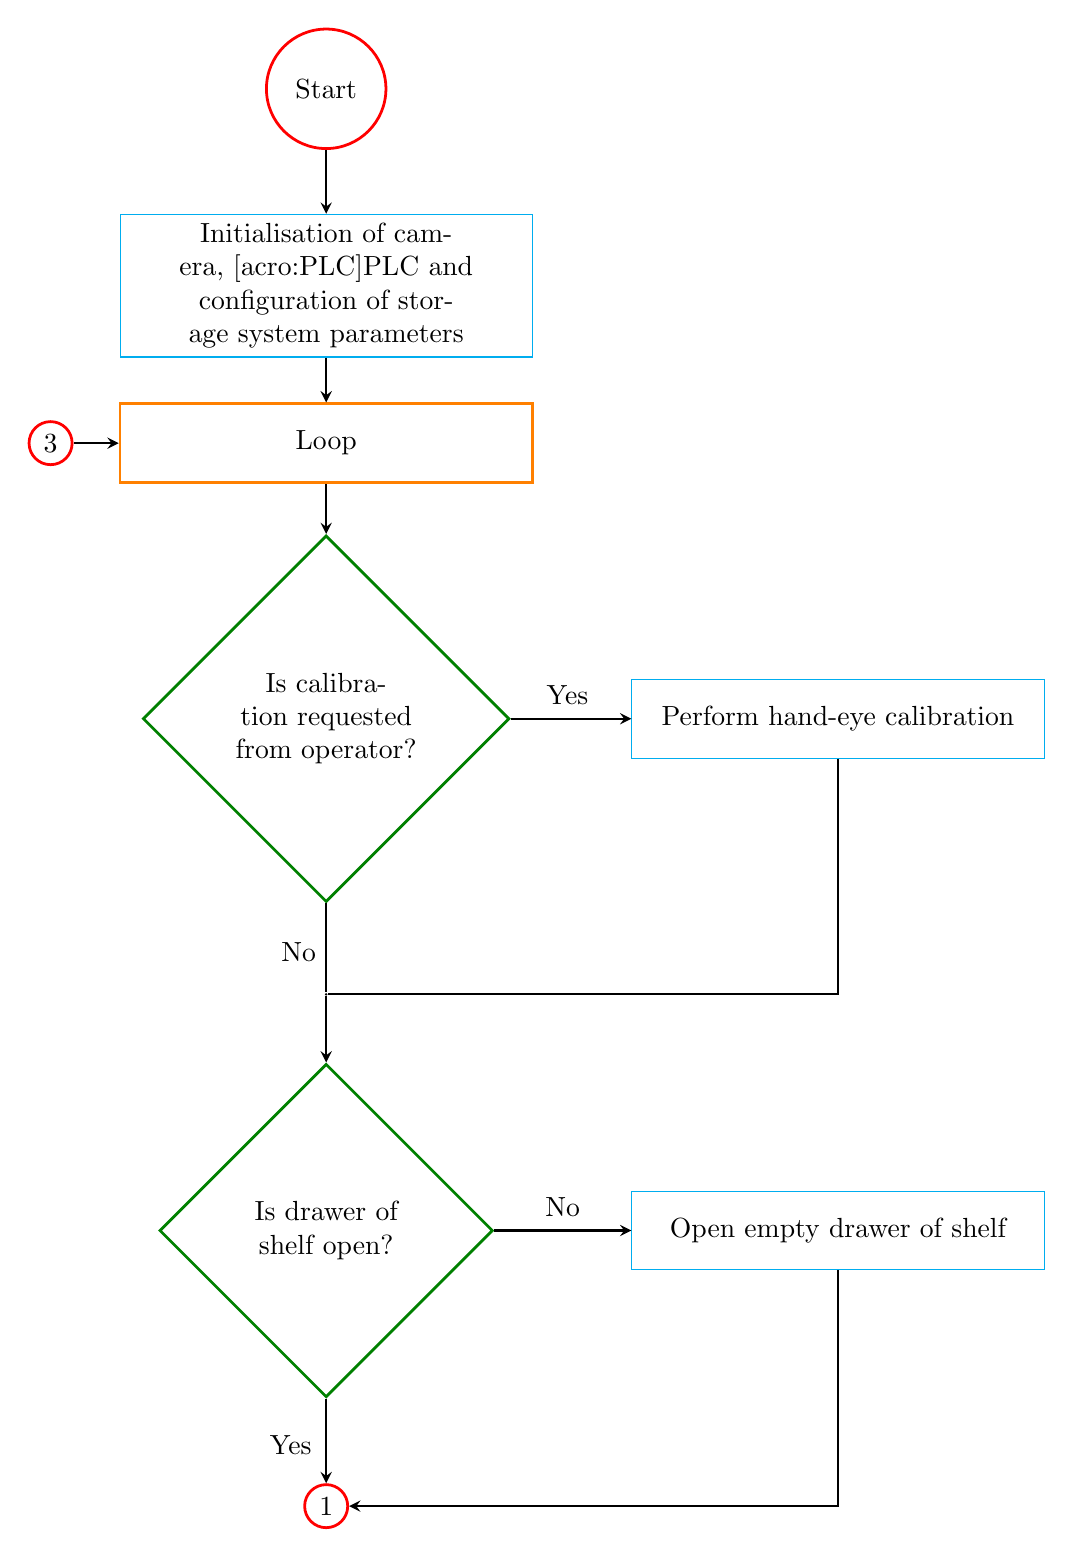
\begin{tikzpicture}[node distance=3.5cm]
        \node (start) [startstop] {Start};
        \node (proc0) [process, below of=start, yshift=1cm] {Initialisation of camera, \hyperref[acro:PLC]{PLC} and configuration of storage system parameters};
        \node (loop)  [processorange, below of=proc0, yshift=1.5cm] {Loop};
        \node (nodeint) [nodepage, left of=loop] {3};
        \node (dec0) [decision, below of=loop] {Is calibration requested from operator?};
        \node (intersection0) [coordinate, below of=dec0] {};
        \node (proc1) [process, right of=dec0, xshift=3cm] {Perform hand-eye calibration};
        \node (dec1) [decision, below of=intersection0, yshift=0.5cm] {Is drawer of shelf open?};
        \node (proc2) [process, right of=dec1, xshift=3cm] {Open empty drawer of shelf};
        \node (intersection1) [nodepage, below of=dec1] {1};

        \draw [arrow] (start) -- (proc0);
        \draw [arrow] (proc0) -- (loop);
        \draw [arrow] (loop) -- (dec0);
        \draw [arrow] (dec0) -- node[anchor=east, yshift=0.3cm, xshift=0.35cm] {Yes} (proc1);
        \draw [black, thick] (dec0) -- node[anchor=south, yshift=-0.3cm, xshift=-0.35cm] {No} (intersection0);
        \draw [black, thick] (proc1) |- (intersection0);
        \draw [arrow] (intersection0) -- (dec1);
        \draw [arrow] (dec1) -- node[anchor=east, yshift=0.3cm, xshift=0.35cm] {No} (proc2);
        \draw [arrow] (dec1) -- node[anchor=south, yshift=-0.3cm, xshift=-0.45cm] {Yes} (intersection1);
        \draw [arrow] (proc2) |- (intersection1);
        \draw [arrow] (nodeint) -- (loop);
    \end{tikzpicture} \\

    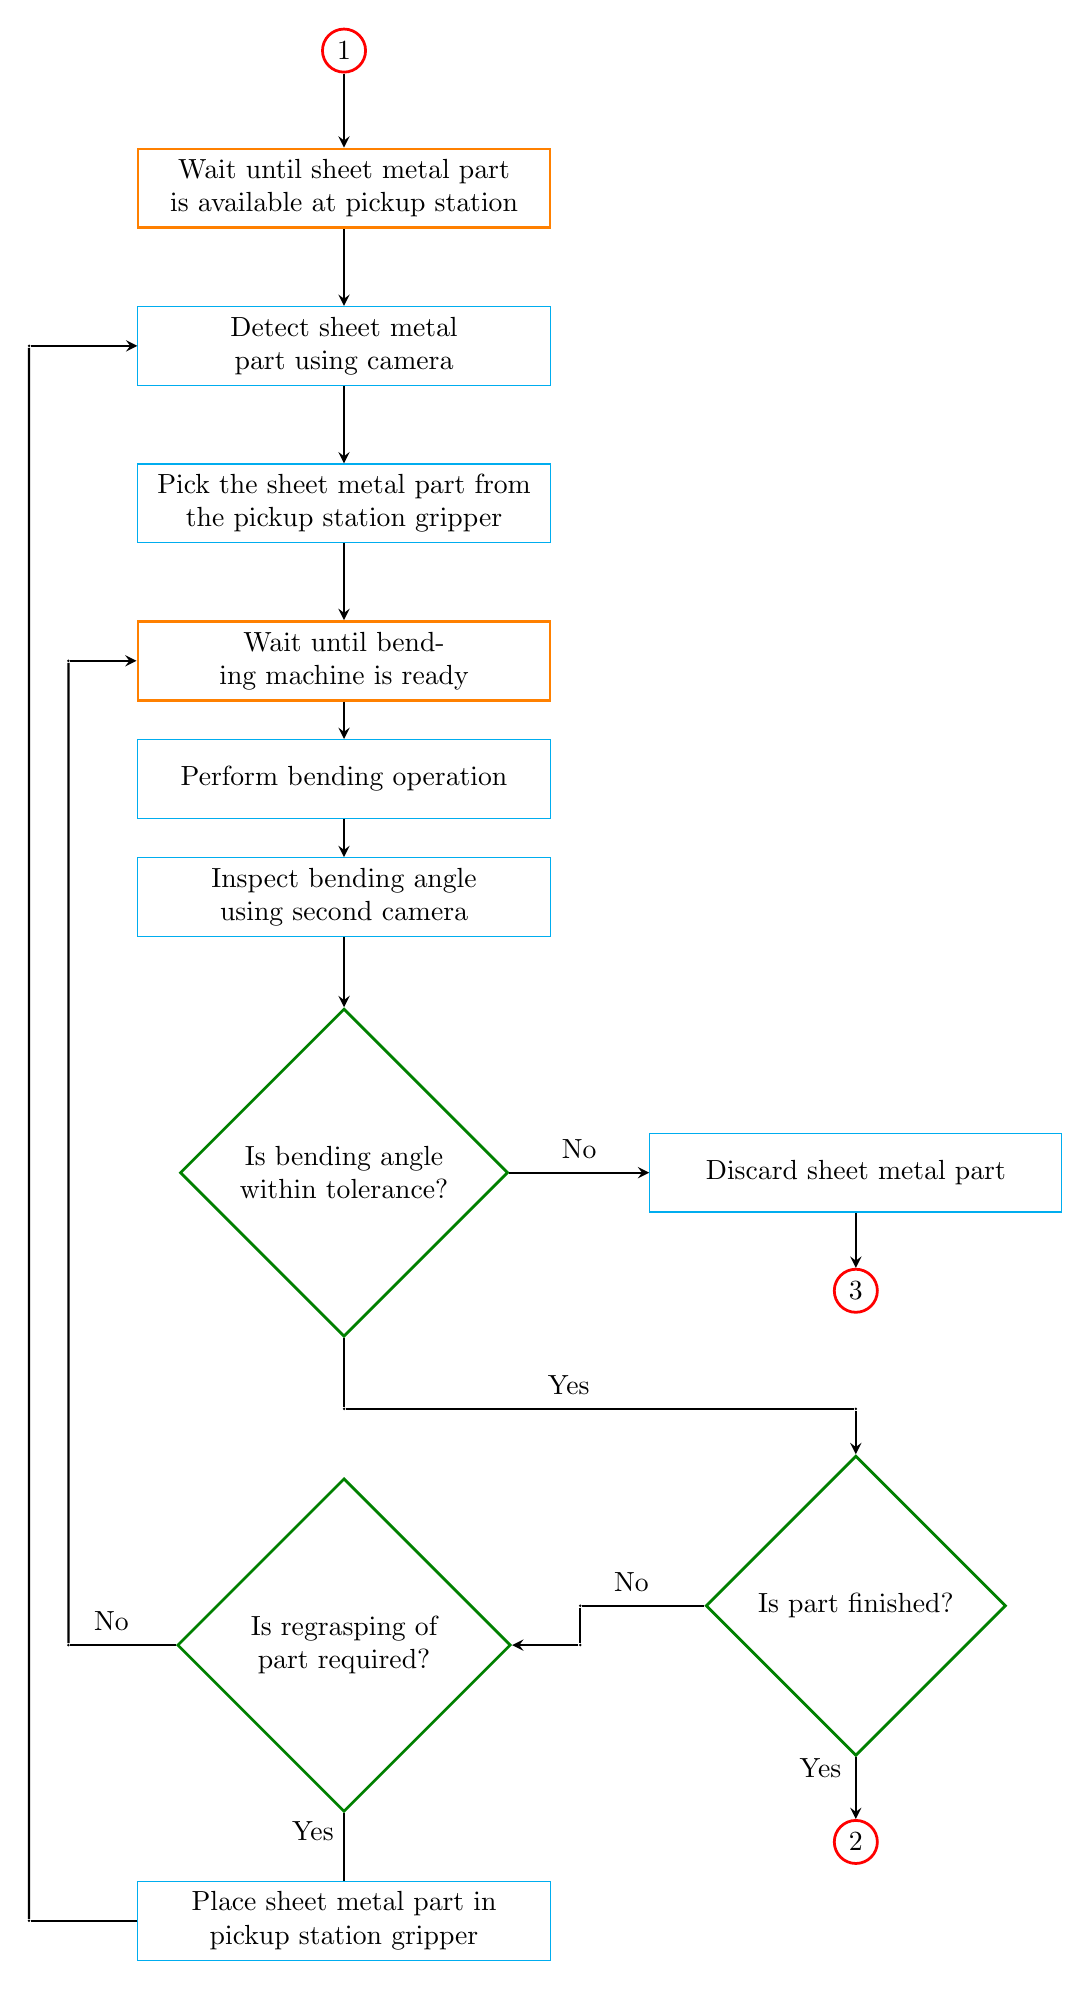
\begin{tikzpicture}[node distance=3.5cm]
        \node (intersection1) [nodepage] {1};
        \node (proc3) [processorange, below of=intersection1, yshift=1.75cm] {Wait until sheet metal part is available at pickup station};
        \node (proc4) [process, below of=proc3, yshift=1.5cm] {Detect sheet metal part using camera};
        \node (point7) [coordinate, left of=proc4, xshift=-0.5cm] {};
        \node (proc5) [process, below of=proc4, yshift=1.5cm] {Pick the sheet metal part from the pickup station gripper};
        \node (proc6) [processorange, below of=proc5, yshift=1.5cm] {Wait until bending machine is ready};
        \node (point5) [coordinate, left of=proc6] {};
        \node (proc7) [process, below of=proc6, yshift=2cm] {Perform bending operation};
        \node (proc8) [process, below of=proc7, yshift=2cm] {Inspect bending angle using second camera};
        \node (dec2) [decision, below of=proc8, yshift=0cm] {Is bending angle within tolerance?};
        \node (proc9) [process, right of=dec2, xshift=3cm] {Discard sheet metal part};
        \node (intersection2) [nodepage, below of=proc9, yshift=2cm] {3};
        \node (point1) [coordinate, below of=dec2, yshift=0.5cm] {};
        \node (point2) [coordinate, right of=point1, xshift=3cm] {};
        \node (dec3) [decision, below of=point2, yshift=1cm] {Is part finished?};
        \node (intersection3) [nodepage, below of=dec3, yshift=0.5cm] {2};
        \node (point3) [coordinate, left of=dec3, xshift=0cm] {};
        \node (point4) [coordinate, below of=point3, yshift=3cm] {};
        \node (dec4) [decision, left of=point4, xshift=0.5cm] {Is regrasping of part required?};
        \node (point6) [coordinate, left of=dec4] {};
        \node (point8) [process, below of=dec4, yshift=0cm] {Place sheet metal part in pickup station gripper};
        \node (point9) [coordinate, left of=point8, xshift=-0.5cm] {};


        \draw [arrow] (intersection1) -- (proc3);
        \draw [arrow] (proc3) -- (proc4);
        \draw [arrow] (proc4) -- (proc5);
        \draw [arrow] (proc5) -- (proc6);
        \draw [arrow] (proc6) -- (proc7);
        \draw [arrow] (point5) -- (proc6.west);
        \draw [arrow] (proc7) -- (proc8);
        \draw [arrow] (proc8) -- (dec2);
        \draw [arrow] (dec2) -- node[anchor=east, yshift=0.3cm, xshift=0.35cm] {No} (proc9);
        \draw [arrow] (proc9) -- (intersection2);
        \draw [black, thick] (dec2) -- (point1);
        \draw [black, thick] (point1) -- node[anchor=east, yshift=0.3cm] {Yes} (point2);
        \draw [arrow] (point2) -- (dec3);
        \draw [black, thick] (dec3) -- node[anchor=west, yshift=0.3cm, xshift=-0.5cm] {No} (point3);
        \draw [black, thick] (point3) -- (point4);
        \draw [arrow] (point4) --  (dec4);
        \draw [black, thick] (point5) -- (point6);
        \draw [black, thick] (point6) -- node[anchor=west, yshift=0.3cm, xshift=-0.5cm] {No} (dec4);
        \draw [black, thick] (dec4) -- node[anchor=east, yshift=0.2cm, xshift=0cm] {Yes} (point8);
        \draw [black, thick] (point8) -- (point9);
        \draw [black, thick] (point9) -- (point7);
        \draw [arrow] (point7) --  (proc4.west);

        % \draw [arrow] (dec2) -- node[anchor=south, yshift=-0.1cm, xshift=-0.45cm] {Yes} (dec3);
        \draw [arrow] (dec3) -- node[anchor=south, yshift=0cm, xshift=-0.45cm] {Yes} (intersection3);


    \end{tikzpicture} \\

    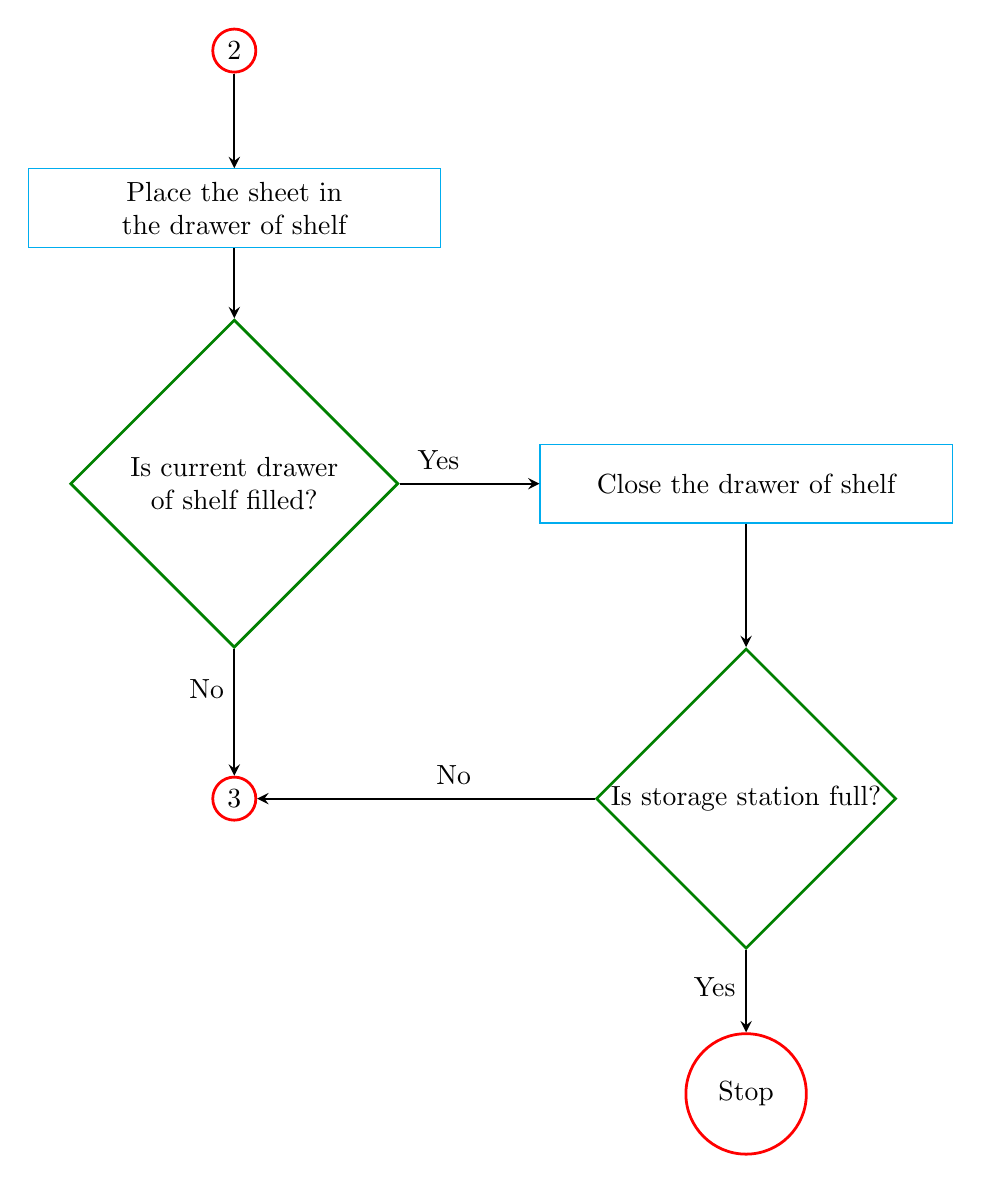
\begin{tikzpicture}[node distance=2cm]
        \node (intersection3) [nodepage] {2};
        \node (proc10) [process, below of=intersection3] {Place the sheet in the drawer of shelf};
        \node (dec5) [decision, below of=proc10, yshift=-1.5cm] {Is current drawer of shelf filled?};
        \node (proc11) [process, right of=dec5, xshift=4.5cm] {Close the drawer of shelf};
        \node (dec6) [decision, below of=proc11, yshift=-2cm] {Is storage station full?};
        \node (intersection4) [nodepage, below of=dec5, yshift=-2cm] {3};
        \node (stop) [startstop, below of=dec6, yshift=-1.75cm] {Stop};


        \draw [arrow] (intersection3) -- (proc10);
        \draw [arrow] (proc10) -- (dec5);
        \draw [arrow] (proc11) -- (dec6);
        \draw [arrow] (dec5) -- node[anchor=east, yshift=0.3cm, xshift=0cm] {Yes} (proc11);
        \draw [arrow] (dec5) -- node[anchor=east, yshift=0.3cm, xshift=0cm] {No} (intersection4);
        \draw [arrow] (dec6) -- node[anchor=west, yshift=0.3cm, xshift=0cm] {No} (intersection4);
        \draw [arrow] (dec6) -- node[anchor=south, yshift=-0.2cm, xshift=-0.4cm] {Yes} (stop);


    \end{tikzpicture} \\
    \\
    \caption{Control program flowchart of robot unit} \label{tab:flowchart}
\end{longtable}


In teach pendant program tree, pose describes a frame transformation in 3D space \textit{i.e.} the three coordinates (x,y,z) and euler angles (R,P,Y) \textit{w.r.t.}
reference frame.



\section{Camera 1: Feature Detection}
Robotic camera has to do three tasks during the whole operation in the robotic workcell. These include:
\begin{enumerate}
    \item Auto-calibrate itself when requested by operator to improve the bending quality.
    \item Find the pose of subsystems in the robotic workcell \textit{i.e.} unloading station, drawers of shelf and the bending machine.
    \item Detect the sheet metal part in the unloading station proper. Then send the sheet poses to the robot via ethernet. For more information about the communication setup between \hyperref[acro:VISOR]{VISOR}\textsuperscript{\textregistered} and robot, see subsection \ref{subsec:computer-vision}.
\end{enumerate}



In teach pendant program tree, a pose describes a frame transformation in \hyperref[acro:3D]{3D} space \textit{i.e.} the three coordinates (x,y,z) and euler angles (R,P,Y) \textit{w.r.t.} reference frame. If no reference frame is defined for the pose in the \hyperref[acro:GUI]{GUI}, then it is automatically set \textit{w.r.t.} world frame.

\begin{figure}[h]
    \centering
    \includegraphics[width=\textwidth]{figures/job-configuration.png}
    \caption{Job configuration for the robotic camera}
    \label{fig:job-configuration-robotic}
\end{figure}

For a test specimen sheet metal type variant, a number of jobs are created during the camera configuration to fulfill the above-mentioned tasks.
Figure \ref{fig:job-configuration-robotic} shows the job configuration for all the jobs in the robotic camera.
After calibration, a working distance of 300.0 mm is set. This is the best operational distance for the camera from an object which has to be detected. The shutter speed varies from 15.0 ms, 30.0 ms, 45.0 ms, 60.0 ms, 75.0 ms and 90.0 ms. Thus, the camera takes a total of six captures with different shutter speed setting, if the default 60.0 ms shutter speed is unable to detect the sheet. A lower shutter speed value means less light will pass through the camera lens and the image will be darker in comparison to higher shutter speed settings. This setting is set in the cycle time tab.
Internal illumination is not used because of a large working distance. An external light is used to illuminate the sheet surface which is always on.


\begin{figure}[h]
    \centering
    \includegraphics[width=\textwidth]{figures/robotic-detection.png}
    \caption{Using robotic camera for sheet detection (left) and marker detection (right)}
    \label{fig:robotic-detection}
\end{figure}

Mainly two detector methods are used by the robotic camera as shown in figure \ref{fig:robotic-detection}. These are detector contour and detector target mark 3D. \textbf{Detector Contour} locate and count objects by contours. An interesting region on the sheet metal part is marked for contouring. 
\textbf{Detector Target Mark 3D} locate objects in space using standardized markers (3D).
Whenever an object is detected by the camera, pose value of object is generated in world frame and sent over to the robot using telegram.

\section{Camera 2: Inspection and Quality Control}
Inspection camera has to measure the bending angle of the bent sheet metal part. KR1410 brings the bent sheet to the inspection camera. Correct alignment of the bent sheet by the robot is particularly important for inspection. The detection of edges of sheet takes place in the inspection process by the reflection of camera's internal red light around the sheet edges. Since the edges of the sheet could have different surface structure or have impurities over them, angle tolerance needs to be setup for each inspection. Separate job is to be created for each inspection.

\begin{figure}[h]
    \centering
    \includegraphics[width=\textwidth]{figures/job-configuration-object.png}
    \caption{Job configuration for the object camera}
    \label{fig:job-configuration-object}
\end{figure}

For the inspection of bent sheet, a job is created with the configuration as shown in figure \ref{fig:job-configuration-object}. A working distance is set in the range of 90 mm to 130 mm for each inspection job. The is the optimum distance for the inspection as the object needs to fully illuminated by the red light. The shutter speed is set to 1.0 ms. This means the camera lens will open only for a duration of 1.0 ms. Thus, only the red light is used to capture the bent sheet image and there is no issue of ambient light. Internal illumination is required in this case.
Only images processing is required by this camera.

\begin{figure}[h]
    \centering
    \includegraphics[width=0.6\textwidth]{figures/measurement-detector.png}
    \caption{Detectors in Inspection Camera for angle measurement}
    \label{fig:measurement-detector}
\end{figure}

From the figure \ref{fig:measurement-detector}, the inspection camera uses an alignment detector, four caliper detectors and one results processing of caliper detectors to calculate the angle.
\textbf{Alignment} detector uses a reference detection in the image and aligns the other detectors \textit{w.r.t.} \textbf{Alignment} detector. 
Four \textbf{Detector Caliper} are used to measure the distance between the edges when the detector transitions from dark to light and again from light to dark. Thus two probes, antiparallel setup is used. Angle measurement is of interest, so four points are detected on the sheet. 
Now, the fifth detector, \textbf{Result Processing: Math}, is used to first calculate the angle between two points lying on the same edge of sheet \textit{v}1. Similarly, another pair of points are used to get the angle between them \textit{v}2. Finally, the angle between these \textit{v}1 and \textit{v}2 is calculated to get the final bending angle \textit{v}3. \textit{v}4 is calculated by checking if the angle is within the tolerances. \textit{v}5 is set to \textit{v}3 if the output of \textit{v}4 is true, otherwise it is set to 0. The PLC receives the output \textit{v}4 and \textit{v}5 of detector number 5, \textbf{Result Processing}.


\section{Web Interface Design}

\begin{figure}[h]
    \centering
    \includegraphics[width=1\textwidth]{figures/webui/webui0.png}
    \caption{Web User Interface}
    \label{fig:web-ui}
\end{figure}

\subsection{Viewer}
\label{subsec:web-ui-viewer}


\subsection{Auto connection}
\label{subsec:web-ui-auto-connection}


\subsection{Robot URDF Visualization}
\label{subsec:web-ui-urdf-visualization}

\subsection{Interactive Marker}
\label{subsec:web-ui-interactive-marker}


\subsection{ROS Control Panel}
\label{subsec:web-ui-ros-control}
Simulation Mode, Robot mode


\begin{figure}[h]
    \centering
    \includegraphics[width=1\textwidth]{figures/webui/web-ui-preview.png}
    \caption{Web User Interface previewing task execution}
    \label{fig:web-ui-preview}
\end{figure}

\subsubsection{Joint Slider}
\label{subsubsec:web-ui-joint-slider}

\subsubsection{Current Pose}
\label{subsubsec:web-ui-current-pose}

\subsubsection{View and Manipulation}
\label{subsubsec:web-ui-view-manipulation}

\subsubsection{IM Size}
\label{subsubsec:web-ui-im-size}


\subsubsection{Buttons}
\label{subsubsec:web-ui-buttons}

\subsection{Saving and loading path}
\label{subsec:web-ui-saving-path}





\chapter{System Integration and Testing}
\label{chap:testing}

\setcounter{section}{0}
\setcounter{subsection}{0}

\section{Calibration}
\label{sec:calibration}

Calibration is a crucial procedure in the development of 
an automated robotic workcell, ensuring that all components
operate accurately and in harmony. Robot calibration ensures that the Kassow robot can accurately position its end effector for loading, bending, and unloading metal sheets. This involves:

\subsection{Kinematic Calibration}
\label{subsec:kinematic-calibration}
It refers to the KR1410's kinematic model which needs to correct any discrepancies between the theoretical model and the actual hardware. This includes measuring and compensating for joint offsets, link lengths, and joint angles. 
The KR1410 is already calibrated from the factory and does not need to be setup. Though in simulation, robot kinematic model is generated from the URDF and needs to be updated to match the real hardware. Figure \ref{fig:tcp} shows the kinematic model of KR1410 and also the TCP link which is set at 216 mm from the TFC.

\begin{figure}[h]
    \centering
    \includegraphics[width=1\textwidth]{6. System Integration and Testing/6.2 Calibration Procedures/tcp.PNG}
    \caption{Kinematic model of KR1410 in RViz}
    \label{fig:tcp}
\end{figure}

\subsection{Tool Center Point (TCP) Calibration}
\label{subsubsec:tcp-calibration}
\begin{itemize}
    \item \textbf{}: Determining the exact position of the end effector or tool relative to the robot’s last joint. This is crucial for precise manipulation of metal sheets.
    \item \textbf{Workspace Calibration}: Defining the robot's operational workspace and ensuring that all tasks are performed within this defined area, avoiding collisions and ensuring smooth operation.
\end{itemize}

\begin{figure}[h]
    \centering
    \begin{subfigure}{0.48\textwidth}
        \centering
        \includegraphics[width=\textwidth, angle=0]{figures/001calibration/calibration-process-left.jpeg} % Replace with your image file
        \label{fig:calibration-process-left}
    \end{subfigure}\hspace{0cm}
    \begin{subfigure}{0.48\textwidth}
        \centering
        \includegraphics[width=\textwidth, angle=0]{figures/001calibration/calibration-process-right.jpeg} % Replace with your image file
        \label{fig:calibration-process-right}
    \end{subfigure}
    \caption{KR1410 subprogram to perform calibration automatically}
    \label{fig:auto-calibration-process}
\end{figure}

\subsection{Camera Calibration}
The "Hand-Eye calibration (Robotics)" calibration method is used to determine the
reference between "Hand" (TCP) and "Eye" Camera coordinate system
(position and orientation) when the VISOR\textsuperscript{\textregistered} is attached to the gripper.
This allows different image acquisition positions and still to output the object positions
in robot coordinates directly from the camera.
\cite[page 102]{visor_user_manual}

Camera calibration is essential for the accurate detection of metal sheets and measurement of bending angles. The process involves:

\begin{itemize}
    \item \textbf{Intrinsic Calibration}: Determining the camera's internal parameters, such as focal length, optical center, and lens distortion. This is typically achieved using a calibration target (e.g., a checkerboard pattern) and specialized software tools.
    \item \textbf{Extrinsic Calibration}: Establishing the camera's position and orientation relative to the robot or the workcell. This involves aligning the camera's coordinate system with the robot’s coordinate system to ensure accurate detection and measurement.
\end{itemize}

\subsection{Sensor Calibration}
Laser sensor is added to the bending machine to measure the distance between the tool and die with the reproducibility in the range of 10\textmu m. This sensor help in coordinating the bending timings between the bending machine and the robot. This sensor also requires a baseline or zero point to eliminate any offsets or biases in their readings.

\subsection{Calibration Procedures}

The calibration process is automated within the robot program
such that operator could request to re-calibrate the camera w.r.t
robot TCP from the touch panel. This allows to update the image quality as it degrades over time. 
The robot finishes the current
bending operation and then in next cycle, start with the auto-calibration.

\begin{figure}[h]
    \centering
    \begin{subfigure}{0.32\textwidth}
        \centering
        \includegraphics[width=\textwidth]{figures/001calibration/calibration.png}
    \end{subfigure}\hspace{0cm}
    \begin{subfigure}{0.32\textwidth}
        \centering
        \includegraphics[width=\textwidth]{figures/001calibration/calibration1.png}
    \end{subfigure}
    \vspace{0.1cm}
    \begin{subfigure}{0.32\textwidth}
        \centering
        \includegraphics[width=\textwidth]{figures/001calibration/calibration2.PNG}
    \end{subfigure}
    \vspace{0.1cm}
    \begin{subfigure}{0.32\textwidth}
        \centering
        \includegraphics[width=\textwidth]{figures/001calibration/calibration3.png}
    \end{subfigure}\hspace{0cm}
    \begin{subfigure}{0.32\textwidth}
        \centering
        \includegraphics[width=\textwidth]{figures/001calibration/calibration4.png}
    \end{subfigure}
    \begin{subfigure}{0.32\textwidth}
        \centering
        \includegraphics[width=\textwidth]{figures/001calibration/calibration5.PNG}
    \end{subfigure}
    \begin{subfigure}{0.32\textwidth}
        \centering
        \includegraphics[width=\textwidth]{figures/001calibration/calibration6.png}
    \end{subfigure}\hspace{0cm}
    \begin{subfigure}{0.32\textwidth}
        \centering
        \includegraphics[width=\textwidth]{figures/001calibration/calibration7.png}
    \end{subfigure}
    \begin{subfigure}{0.32\textwidth}
        \centering
        \includegraphics[width=\textwidth]{figures/001calibration/calibration8.PNG}
    \end{subfigure}

    \caption{Acquiring images for the calibration process}
    \label{fig:calibration-steps}
\end{figure}

\begin{figure}
    \centering
    \footnotesize
    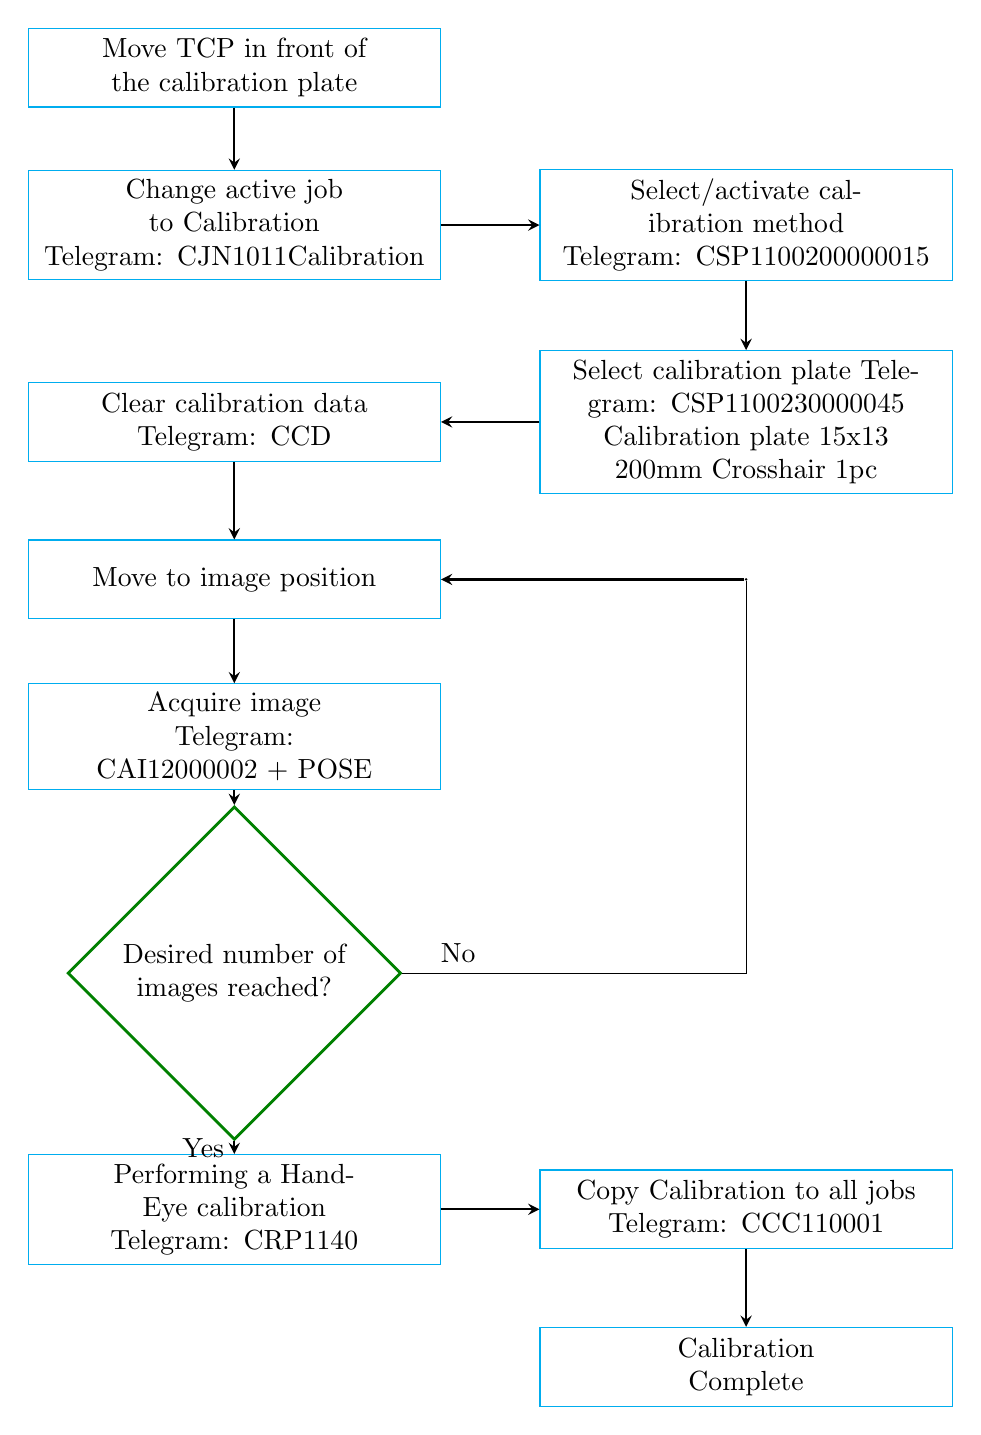
\begin{tikzpicture}[node distance=2cm]
    
        % Nodes
        \node (ready) [process] {Move TCP in front of the calibration plate};
        \node (job) [process, below of=ready] {Change active job to Calibration\\ Telegram: CJN1011Calibration};
        \node (start) [process, right of=job, xshift=4.5cm] {Select/activate calibration method\\ Telegram: CSP1100200000015};
        \node (plate) [process, below of=start,yshift=-0.5cm] {Select calibration plate Telegram: CSP1100230000045\\ Calibration plate 15x13 200mm Crosshair 1pc};
        \node (clear) [process, left of=plate,xshift=-4.5cm] {Clear calibration data \\ Telegram: CCD};
        \node (move) [process, below of=clear] {Move to image position};
        \node (point) [coordinate, right of=move, xshift=4.5cm] {};
        \node (acquire) [process, below of=move] {Acquire image \\ Telegram: CAI12000002 + POSE};
        \node (decision) [decision, below of=acquire, yshift=-1cm] {Desired number of images reached?};
        \node (calibrate) [process, below of=decision, yshift=-1cm] {Performing a Hand-Eye calibration \\ Telegram: CRP1140};
        \node (copy) [process, right of=calibrate,xshift=4.5cm] {Copy Calibration to all jobs \\ Telegram: CCC110001};
        \node (complete) [process, below of=copy] {Calibration\\ Complete};

        
        % Arrows
        \draw [arrow] (ready) -- (job);
        \draw [arrow] (job) -- (start);
        \draw [arrow] (start) -- (plate);
        \draw [arrow] (plate) -- (clear);
        \draw [arrow] (clear) -- (move);
        \draw [arrow] (move) -- (acquire);
        \draw [arrow] (acquire) -- (decision);
        \draw [arrow] (decision) -- node[anchor=east] {Yes} (calibrate);
        \draw [-] (decision) -| node[anchor=west, xshift=-4cm, yshift=0.25cm] {No} (point);
        \draw [arrow] (point) -- (move);
        \draw [arrow] (calibrate) -- (copy);
        \draw [arrow] (copy) -- (complete);

        
    \end{tikzpicture}
    \caption{Hand-eye calibration procedure using telegram}
    \label{fig:calib-graph}
\end{figure}


The calibration process involves several systematic steps:

\begin{enumerate}
    \item \textbf{Setup Calibration Targets}: Place calibration targets within the robot's workspace and at specific positions that the cameras will observe.
    \item \textbf{Data Collection}: Use the robot and cameras to collect data from the calibration targets. This includes moving the robot through its range of motion and capturing images from different angles.
    \item \textbf{Parameter Estimation}: Use calibration software to estimate the parameters of the robot’s kinematic model, the intrinsic and extrinsic parameters of the cameras, and the characteristics of any other sensors.
    \item \textbf{Validation}: Verify the calibration by performing tasks that require high precision and checking the accuracy of the results. Adjust calibration parameters as needed based on validation results.
    \item \textbf{Documentation}: Record the calibration parameters and procedures for future reference and troubleshooting.
\end{enumerate}


\subsection{Workspace Calibration}
\label{subsec:workspace-calibration}




\FloatBarrier  % Force all figures of the first section to be placed before the next section

\section{Integration Tests}
\label{sec:integration}
\subsection{Sheet Pickup}
\label{subsec:sheet-pickup}

\begin{figure}[h]
    \centering
    \begin{subfigure}[b]{0.48\textwidth}
        \centering
        \includegraphics[width=\textwidth]{figures/sheet-pickup/scan.png}
        \caption{Scan sheet pattern using contour detector}
        \label{subfig:sheet-scan}
    \end{subfigure}\hspace{0.1cm}
    \begin{subfigure}[b]{0.48\textwidth}
        \centering
        \includegraphics[width=\textwidth]{figures/sheet-pickup/taken.png}
        \caption{collect the sheet}
        \label{subfig:sheet-taken}
    \end{subfigure}
    \caption{Sheet pickup using robotic gripper}
    \label{fig:sheet-pickup}
\end{figure}

\begin{figure}[h]
    \centering
    \includegraphics[width=\textwidth]{figures/sheet-pickup/sensoconfig.PNG}
    \caption{detection and transfer of sheet pose using telegram (SensoConfig)}
    \label{fig:sensoconfig-pattern}
\end{figure}


\begin{figure}[h]
    \centering
    \begin{subfigure}[b]{0.48\textwidth}
        \centering
        \includegraphics[width=\textwidth]{figures/sheet-pickup/camera-align.png}
        \caption{align camera}
        \label{subfig:sheet-scan}
    \end{subfigure}\hspace{0.1cm}
    \begin{subfigure}[b]{0.48\textwidth}
        \centering
        \includegraphics[width=\textwidth]{figures/sheet-pickup/sheet-pose.png}
        \caption{send sheet pose to pickup the sheet}
        \label{subfig:sheet-taken}
    \end{subfigure}
    \caption{Sheet pattern detection using detector contour}
    \label{fig:sheet-scanning}
\end{figure}

\begin{figure}[h]
    \centering
    \begin{subfigure}[b]{0.32\textwidth}
        \centering
        \includegraphics[width=\textwidth]{figures/sheet-pickup/sheet-placement01.png}
        \caption{Go to unloading station gripper}
        \label{subfig:sheet-placement01}
    \end{subfigure}\hspace{0.1cm}
    \begin{subfigure}[b]{0.32\textwidth}
        \centering
        \includegraphics[width=\textwidth]{figures/sheet-pickup/sheet-placement02.png}
        \caption{transfer sheet to unloading station gripper}
        \label{subfig:sheet-placement02}
    \end{subfigure}\hspace{0.1cm}
    \vspace{1cm}
    \begin{subfigure}[b]{0.32\textwidth}
        \centering
        \includegraphics[width=\textwidth]{figures/sheet-pickup/sheet-placement03.png}
        \caption{Scan sheet pattern and align camera}
        % \vspace{-0.45cm}
        \label{subfig:sheet-placement03}
    \end{subfigure}\hspace{0.1cm}
    \begin{subfigure}[b]{0.32\textwidth}
        \centering
        \includegraphics[width=\textwidth]{figures/sheet-pickup/sheet-placement04.png}
        \caption{Scan again for sheet detection}
        \label{subfig:sheet-placement04}
    \end{subfigure}\hspace{0.1cm}
    \vspace{0.75cm}
    \begin{subfigure}[b]{0.32\textwidth}
        \centering
        \includegraphics[width=\textwidth]{figures/sheet-pickup/sheet-placement05.png}
        \caption{Grasp sheet from unloading station gripper}
        \label{subfig:sheet-placement05}
    \end{subfigure}\hspace{0.1cm}
    \begin{subfigure}[b]{0.32\textwidth}
        \centering
        \includegraphics[width=\textwidth]{figures/sheet-pickup/sheet-placement06.png}
        \caption{Move out}
        \label{subfig:sheet-placement06}
        \vspace{0.45cm}
    \end{subfigure}\hspace{0.1cm}
    \caption{Regrasping bent sheet from a different position before placement in drawer}
    \label{fig:sheet-pickup-before-placement}
\end{figure}

\FloatBarrier  % Force all figures of the first section to be placed before the next section

\subsection{Bending Operation}
\label{subsec:bending-operation}
% Bending operations

The test part undergoes a sequence of six bendings, with different angles and setups. Specifically, bending operations 1, 5, and 6 are performed at bending station 1 and undergoes a bending of 90° angle, whereas bending operations 2 and 3 are performed at bending station 2 with a bending of 135°, and the fourth bending operation is simply done to flatten the sheet metal part.

The first step before the bending for all bending operations is the correct alignment of the part in the backgauges of the bending machine. The bending machine program is automatically set by the terminal operating robot. Once the correct sequence is selected in the terminal of the bending machine, PLC send a signal to the KR1410 robot which gives permission to align the sheet in the backgauges.
Then only the KR1410 arm secures the part in the backgauges of the bending machine.

\begin{figure}[h]
    \centering
    \begin{subfigure}[b]{0.32\textwidth}
        \centering
        \includegraphics[width=\textwidth]{figures/bending/bending1-002.png}
        \caption{Go to bending station 1}
        \label{subfig:bending1-before}
    \end{subfigure}\hspace{0.1cm}
    \begin{subfigure}[b]{0.32\textwidth}
        \centering
        \includegraphics[width=\textwidth]{figures/bending/bending1-003.png}
        \caption{bend the sheet metal part}
        \label{subfig:bending1}
    \end{subfigure}\hspace{0.1cm}
    \begin{subfigure}[b]{0.32\textwidth}
        \centering
        \includegraphics[width=\textwidth]{figures/bending/bending1-001.png}
        \caption{take away the bent sheet}
        \label{subfig:bending1-after}
    \end{subfigure}\hspace{0.1cm}
    \caption{Bending operation number 1 at bending station 1}
    \label{fig:bending-operation-1}
\end{figure}

\begin{figure}[h]
    \centering
    \begin{subfigure}[b]{0.32\textwidth}
        \centering
        \includegraphics[width=\textwidth]{figures/bending/bending2-003.png}
        \caption{Go to bending station 2}
        \label{subfig:bending2-before}
    \end{subfigure}\hspace{0.1cm}
    \begin{subfigure}[b]{0.32\textwidth}
        \centering
        \includegraphics[width=\textwidth]{figures/bending/bending2-001.png}
        \caption{bend the sheet metal part}
        \label{subfig:bending2}
    \end{subfigure}\hspace{0.1cm}
    \begin{subfigure}[b]{0.32\textwidth}
        \centering
        \includegraphics[width=\textwidth]{figures/bending/bending2-002.png}
        \caption{take away the bent sheet}
        \label{subfig:bending2-after}
    \end{subfigure}\hspace{0.1cm}
    \caption{Bending operation number 2 at bending station 2}
    \label{fig:bending-operation-2}
\end{figure}


Figure \ref{fig:bending-operation-1} shows the transfer of sheet metal part to the first bending station where a 90° bend is performed. The handling robot secures the sheet first. A signal is sent by KR1410 robot to PLC to start bending. The robot opens the gripper as soon as the tool of the bending machine hits the sheet. The sheet is secured by the bending machine and the robot moves to a different pose. From there, the robot moves back to the bent part and grip it. Another signal is sent to PLC to move the tool upwards. Once the tool is clear of the part, robot goes to the inspection camera for angle measurement. Bending machine open height measurement laser sensor is responsible for the timings of the opening and closing of bending machine signals. It helps in making robot work together with the bending machine and avoid any collision.


Figures \ref{fig:bending-operation-2} and \ref{fig:bending-operation-3} shows the bending of part at bending station 2. The process is similar to the first bending. The robot leaves the part during bending and regrip it once the bending is complete. For bending number 3, an inspection is not done, because the bending is done very close to the edge, and the small edge is not measurable by the inspection camera.


\begin{figure}[h]
    \centering
    \begin{subfigure}[b]{0.32\textwidth}
        \centering
        \includegraphics[width=\textwidth]{figures/bending/bending3-001.png}
        \caption{Go to bending station 2}
        \label{subfig:bending3-before}
    \end{subfigure}\hspace{0.1cm}
    \begin{subfigure}[b]{0.32\textwidth}
        \centering
        \includegraphics[width=\textwidth]{figures/bending/bending3-002.png}
        \caption{bend the sheet metal part}
        \label{subfig:bending3}
    \end{subfigure}\hspace{0.1cm}
    \begin{subfigure}[b]{0.32\textwidth}
        \centering
        \includegraphics[width=\textwidth]{figures/bending/bending3-003.png}
        \caption{take away the bent sheet}
        \label{subfig:bending3-after}
    \end{subfigure}\hspace{0.1cm}
    \caption{Bending operation number 3 at bending station 2}
    \label{fig:bending-operation-3}
\end{figure}

\begin{figure}[h]
    \centering
    \begin{subfigure}[b]{0.32\textwidth}
        \centering
        \includegraphics[width=\textwidth]{figures/bending/bending4-001.png}
        \caption{Go to bending station 3}
        \label{subfig:bending4-before}
    \end{subfigure}\hspace{0.1cm}
    \begin{subfigure}[b]{0.32\textwidth}
        \centering
        \includegraphics[width=\textwidth]{figures/bending/bending4-002.png}
        \caption{bend the sheet metal part}
        \label{subfig:bending4}
    \end{subfigure}\hspace{0.1cm}
    \begin{subfigure}[b]{0.32\textwidth}
        \centering
        \includegraphics[width=\textwidth]{figures/bending/bending4-003.png}
        \caption{take away the bent sheet}
        \label{subfig:bending4-after}
    \end{subfigure}\hspace{0.1cm}
    \caption{Bending operation number 4 at bending station 3}
    \label{fig:bending-operation-4}
\end{figure}


Figure \ref{fig:bending-operation-4} shows the bending opertion number 4. Since the tool and die are only used for pressing the sheet to flatten it, the robotic gripper doesn't have to open the gripper during bending. Once the sheet is pressed for a specific duration, tool moves up and the robot takes the part out.  Again the inspection is not done, because there is no warping of sheet in this bending operation.


\begin{figure}[h]
    \centering
    \begin{subfigure}[b]{0.32\textwidth}
        \centering
        \includegraphics[width=\textwidth]{figures/bending/bending5-001.png}
        \caption{Go to bending station 1}
        \label{subfig:bending5-before}
    \end{subfigure}\hspace{0.1cm}
    \begin{subfigure}[b]{0.32\textwidth}
        \centering
        \includegraphics[width=\textwidth]{figures/bending/bending5-002.png}
        \caption{bend the sheet metal part}
        \label{subfig:bending5}
    \end{subfigure}\hspace{0.1cm}
    \begin{subfigure}[b]{0.32\textwidth}
        \centering
        \includegraphics[width=\textwidth]{figures/bending/bending5-003.png}
        \caption{take away the bent sheet}
        \label{subfig:bending5-after}
    \end{subfigure}\hspace{0.1cm}
    \caption{Bending operation number 5 at bending station 1}
    \label{fig:bending-operation-5}
\end{figure}


\begin{figure}[h]
    \centering
    \begin{subfigure}[b]{0.32\textwidth}
        \centering
        \includegraphics[width=\textwidth]{figures/bending/bending6-001.png}
        \caption{Go to bending station 1}
        \label{subfig:bending6-before}
    \end{subfigure}\hspace{0.1cm}
    \begin{subfigure}[b]{0.32\textwidth}
        \centering
        \includegraphics[width=\textwidth]{figures/bending/bending6-003.png}
        \caption{bend the sheet metal part}
        \label{subfig:bending6}
    \end{subfigure}\hspace{0.1cm}
    \begin{subfigure}[b]{0.32\textwidth}
        \centering
        \includegraphics[width=\textwidth]{figures/bending/bending6-002.png}
        \caption{take away the bent sheet}
        \label{subfig:bending6-after}
    \end{subfigure}\hspace{0.1cm}
    \caption{Bending operation number 6 at bending station 1}
    \label{fig:bending-operation-6}
\end{figure}

Bending operation 5 and 6 are performed at bending station 1 as showing in figures \ref{fig:bending-operation-5} and \ref{fig:bending-operation-6} respectively. The process is similar to bending operation 1 as the robot doesn't hold the part during bending. Inspection is done after both bending operations. If after bending operation 6, the angle measurement is within tolerances, the current bending cycle is termed as successful.
\FloatBarrier  % Force all figures of the first section to be placed before the next section

\subsection{Shelf Control}
\label{subsec:shelf-control}

\begin{figure}[h]
    \centering
    \begin{subfigure}[b]{0.32\textwidth}
        \centering
        \includegraphics[width=\textwidth]{figures/shelf-control/reach-handle.jpeg}
        \caption{Reach shelf handle}
        \label{subfig:reach-handle}
    \end{subfigure}\hspace{0.1cm}
    \begin{subfigure}[b]{0.32\textwidth}
        \centering
        \includegraphics[width=\textwidth]{figures/shelf-control/hold-handle.jpeg}
        \caption{grasp handle with gripper}
        \label{subfig:grasp-handle}
    \end{subfigure}\hspace{0.1cm}
    \vspace{1cm}
    \begin{subfigure}[b]{0.32\textwidth}
        \centering
        \includegraphics[width=\textwidth]{figures/shelf-control/open-handle.jpeg}
        \caption{Turn handle 100\textdegree{} to open drawer}
        \vspace{-0.45cm}
        \label{subfig:turn-open}
    \end{subfigure}\hspace{0.1cm}
    \begin{subfigure}[b]{0.32\textwidth}
        \centering
        \includegraphics[width=\textwidth]{figures/shelf-control/open-drawer.jpeg}
        \caption{open drawer}
        \vspace{0.45cm}
        \label{fig:open-drawer}
    \end{subfigure}\hspace{0.1cm}
    \vspace{0.75cm}
    \begin{subfigure}[b]{0.32\textwidth}
        \centering
        \includegraphics[width=\textwidth]{figures/shelf-control/close-handle.jpeg}
        \caption{Turn handle -100\textdegree{} to fix drawer in open position}
        \label{fig:close-handle}
    \end{subfigure}\hspace{0.1cm}
    \begin{subfigure}[b]{0.32\textwidth}
        \centering
        \includegraphics[width=\textwidth]{figures/shelf-control/drawer-opened.jpeg}
        \caption{Robot ready with drawer open}
        \label{subfig:drawer-opened}
    \end{subfigure}\hspace{0.1cm}
    \caption{Opening a shelf drawer for placement of bent sheet metal parts}
    \label{fig:shelf-control}
\end{figure}



\FloatBarrier  % Force all figures of the first section to be placed before the next section



\FloatBarrier  % Force all figures of the first section to be placed before the next section





\chapter{Experimental Results}
\label{chap:results}

\setcounter{section}{0}
\setcounter{subsection}{0}

\section{Performance Evaluation}
\label{sec:performance}
\subsection{Importance of Calibration}
Calibration is fundamental to ensuring the accuracy and reliability of an automated robotic workcell. Proper calibration:

\begin{itemize}
    \item \textbf{Enhances Precision}: Ensures that the robot and sensors operate with high accuracy, essential for tasks like metal sheet bending where precise angles and positions are critical.
    \item \textbf{Improves Consistency}: Reduces variability in operations, leading to consistent product quality and reducing the likelihood of errors.
    \item \textbf{Facilitates Integration}: Ensures that all components of the workcell operate cohesively, enabling smooth integration and coordination.
    \item \textbf{Supports Troubleshooting}: Provides a baseline for identifying and resolving issues that may arise during operation.
\end{itemize}

By establishing rigorous calibration procedures, the automated robotic workcell can achieve optimal performance, ensuring that the bending process is executed with high precision and reliability.

\FloatBarrier  % Force all figures of the first section to be placed before the next section

\section{Setup and Methodology}
\input{7. Experimental Results/7.1 Setup and Methodology/methodology.tex}

\section{Data Collection}
The web user interface allows visualization of the bending process. It also provides control to simulate the robot for the bending process in a simulation environment. This reduces downtime which could be required for the programming and path planning of robot for a new sheet type.

\section{Results and Analysis}
Once the final program has been tested for 50 sheet metal parts and the bending process is evaluated by the project partner, the workcell is moved to the floor space of project partner to start production of parts.

\begin{figure}[h]
    \centering
    \includegraphics[width=\textwidth]{figures/commissioning.jpeg}
    \caption{Commissioning of robotic workcell in project partner floor space}
    \label{fig:commissioning}
\end{figure}

\section*{Chapter 8: Discussion}

\chapter{Conclusion and Future Works}

\setcounter{section}{0}
\setcounter{subsection}{0}

\section{Summary}

\section{Recommendations for Future Research}

% Add all the references here
\addcontentsline{toc}{chapter}{Bibliography}
\setcounter{page}{0}
\pagenumbering{roman}

\printbibliography
\appendix
\renewcommand{\thesection}{A\arabic{section}}

\chapter{Appendix}

\section{Software \& Development Environment Versions}

The following list summarizes the versions of all software used by and required for the
evaluation framework developed in this thesis. Accordingly, the evaluation framework
was only tested to run on these versions.

\begin{itemize}
    \item \textbf{\hyperref[tab:acronyms]{ROS}:} ROS1 Noetic Ninjemys
    \item \textbf{\hyperref[tab:acronyms]{KR} Software Release:} Fire Fly 3
    \item \textbf{Python:} 3.8.10
    \item \textbf{C++:} C++11
    \item \textbf{\hyperref[tab:acronyms]{VISOR\textsuperscript{\textregistered}} \hyperref[tab:acronyms]{PC} Software:} 2.8.2.1
    \item \textbf{\hyperref[tab:acronyms]{ROS} Packages:} ROS packages version is summarized in \textit{package.xml} of the project
    \item \textbf{\hyperref[tab:acronyms]{NodeJS}:} v18.14.0
\end{itemize}

The following list summarizes all development environments used to implement all code
during the course of this thesis:

\begin{itemize}
    \item \textbf{Development \hyperref[tab:acronyms]{OS}:} Ubuntu 20.04.6 LTS (Focal Fossa) for \hyperref[tab:acronyms]{ROS} Simulations and Windows 10 for \hyperref[tab:acronyms]{SENSOPART} Software
    \item \textbf{\hyperref[tab:acronyms]{ROS IDE}:} Visual Studio Code (version 1.91)
    \item \textbf{\hyperref[tab:acronyms]{CBUN IDE}:} Visual Studio Code (version 1.85) Required by \hyperref[tab:acronyms]{KR} for \hyperref[tab:acronyms]{CBUN} Development
\end{itemize}

\newpage

\section{Reduction in Manual Labor}
\section{Cost reduction}

\end{document}